% Created 2015-08-27 木 18:07
\documentclass[11pt,a4paper]{article}
\usepackage[utf8]{inputenc}
\usepackage[dvipdfmx]{graphicx}
\usepackage{ascmac} % 枠付き環境のため
\usepackage{amsmath}
\usepackage{hyperref}
\usepackage{color}
\usepackage{listings,jlisting} % jlistingはtex-live-fullでも入ってない。手動
\usepackage{fancyvrb}

\usepackage{geometry}
\geometry{left=25mm,right=25mm,top=20mm,bottom=20mm}

% \usepackage{courier}
%\usepackage{DejaVuSansMono}
\usepackage[T1]{fontenc}
% \usepackage{lmodern}
% \usepackage{luximono}
\usepackage[scaled=0.85]{beramono}

% \date{\today}

\lstdefinelanguage{SML} {
  keywords = {
    if,then,else,val,rec,let,in,end,fun,fn,exception,handle,raise,
    case,of,datatype,type,op,where,
    ref,struct,structure,signature,sig,functor,before,local,as,
    SOME,NONE
  },
  morecomment=[n]{(*}{*)},%
  ndkeywords={true,false,int,bool,string,char},
  ndkeywordstyle=
}

\lstset{
  language={SML},% プログラミング言語
  basicstyle={\ttfamily\small},% ソースコードのテキストのスタイル
  keywordstyle={\bfseries},% 予約語等のキーワードのスタイル
  commentstyle={\itshape},% コメントのスタイル
  stringstyle={},% 文字列のスタイル
  frame=trlb,% ソースコードの枠線の設定 (none だと非表示)
  numbers=none,% 行番号の表示 (left だと左に表示)
  numberstyle={},% 行番号のスタイル
  xleftmargin=5pt,% 左余白
  xrightmargin=5pt,% 右余白
  keepspaces=true,% 空白を表示する
  mathescape,% $ で囲った部分を数式として表示する ($ がソースコード中で使えなくなるので注意)
  % 手動強調表示の設定
  moredelim=[is][\fontfamily{pcr}\selectfont\itshape]{@/}{/@},
  moredelim=[is][\color{red}]{@r\{}{\}@},
  moredelim=[is][\color{blue}]{@b\{}{\}@},
  moredelim=[is][\color{DarkGreen}]{@g\{}{\}@},
}

\title{SMLコア言語入門}
\author{@no\_maddo}

\begin{document}

\maketitle
\tableofcontents

\setlength{\parskip}{0.1cm}

% \newcommand{\beforesection}[1]{
%  \vspace{-5mm}
% }

% \newcommand{\beforesubsection}[1]{
%  \vspace{-5mm}
% }
\part{Standard MLの世界へようこそ!}
Standard ML(以下SML)の世界へようこそ!\\
SMLは非純粋(副作用、破壊的代入が出来る)な関数型言語の一種です。
Strictな(Cなどと同じ評価順序)評価戦略・静的な(コンパイル時の)型付け・高階関数(関数を操作する関数)など
静的型付けを行う関数型言語として標準的な機能を持つ、MLと呼ばれる歴史ある言語ファミリに属しています。\\
特徴としてはSchemeのように言語の定義が存在します\cite{definition}。
言語の定義が存在すると、言語を処理系を叩いて理解するのではなく、より定式化されたものを対象に理解することが出来ます。

個人的な私見ですが、MLは関数型言語を学ぶための言語として最適です。
わかりやすい言語設計で、特に型システムは関数型言語でも標準的で分かりやすいです。
日本では関数型言語として名前が上がるのはまずHaskell, F\#などかもしれませんが、
これらの型システムもベースはMLで主に用いられるHindley-Milner型システムをベースにしています。

特に言語処理系に興味がある人にとっては、SMLは様々な実験的な処理系が作られてきたのでSMLを
学ぶ意義が大いにあります。
CPS変換によってすべての関数呼び出しが末尾再帰呼出し化される''Standar ML of New Jersey''や
Whole optimized compilerとして有名な、分割コンパイルを諦めて強力な最適化がかかる''MLton'',
定理照明器Isabelle/HOLの開発に用いられているPoly/MLなど。
Type Passingを全面的に利用しようとして夢破れたTILなど、実験的な論文レベルの処理系もたくさんあります。

ぜひこの同人誌を楽しく読むために、SMLのコア言語を学んで下さい。

\section{本チュートリアルの読み方}
このチュートリアルは足早に他のプログラミング言語を何か1つ以上知っている人向けに
SMLのコア言語の書き方をSML/NJを題材に説明します。
関数型言語の知識はあると理解が簡単かと思いますが必要としません。その都度説明します。\\
途中のコラムでは、プログラミング言語マニア向けに言語デザイン・SMLの考え方・他の言語との比較に触れます。
コラムはそこまでの知識では理解できない用語や概念が含まれますので、
分からなければ後で読んでもらうのが良いと思います。

\section{SML/NJ}
\subsection{SML/NJのインストール}
基本的にはインストールの指示に従えば特に困難なくインストールすることが出来ます。\\
\url{http://www.smlnj.org/dist/working/index.html} で最新版を確認してください。
\begin{itemize}
\item Windowsの場合\\
  Windows向けにインストーラが存在します。
  上で示したURLから最新版をクリックし、.msiファイルをダウンロードし、指示に従って下さい。\\
  Windowsではコマンドプロンプト上でSML/NJの対話環境が動くことになります。
  コマンドプロンプトではコピーアンドペーストや基本操作がしづらいと思うので
  Emacsなど他のプログラム上でコマンドプロンプトを実行するようなプログラムが必要かもしれません。
\item Linux系OSの場合\\
  多くのメジャーディストリビューションではパッケージ管理ソフト経由でインストールすることが出来ます。
  執筆現在(2015年10月12日)で最新版は110.78です、パッケージ管理ソフト経由で
  インストールできるコンパイラは古いかもしれませんが基本的には問題ないはずです。
  \lstinline{ml-build}などツールがうまく動かないようならばソースコードからコンパイルして下さい。
\end{itemize}
\subsection{対話環境について}
WIndowsを例に見方を説明します。

\begin{figure}[htbp]
  \centering
  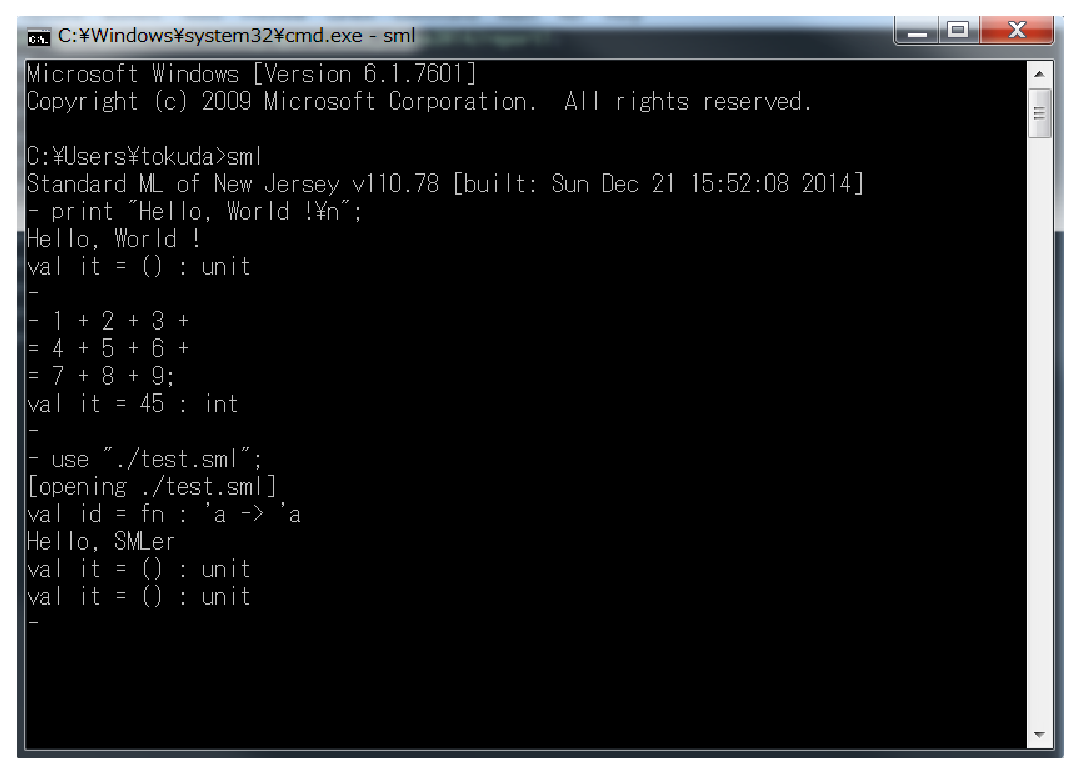
\includegraphics[scale=0.8]{./interactive.eps}
  \caption{対話環境}
  \label{fig:hello}
\end{figure}

コマンドプロンプト上でsmlと入力し、SML/NJを起動しましょう。
その後上の画像のように、\lstinline{print "Hello, World !\n";}と入力してみて下さい。
セミコロンも必ず必要です。画面に正しくプリントされれば成功です!

対話環境の見方を説明します。
\begin{itemize}
\item 各行の最初のハイフン(\lstinline{-})は対話環境が挿入するプロンプトです。
  プログラムの一部ではないので気にしてくて大丈夫です。
\item プログラムが複数行に渡る時は、対話環境がイコール(\lstinline{=})記号を自動的に挿入します。
  これもプログラムの一部ではないので気にしてくて大丈夫です。
\item 行の最後に必要なセミコロン(\lstinline{;})は対話環境に入力が終わったことを
  伝えるために必要な文字です。これがなければずっと対話環境は入力待ちをします。
\item 画面で\lstinline{Hello, World !}の次の行にかかれているように、
  プログラムを実行(これ以降評価と呼びます)すると計算結果とそれの型がプリントされます。
  これによってユーザはインタラクティブに関数を定義し、計算結果を手早く
  確認しながらプログラミングを続けることが出来ます。
\item 対話環境にいちいち打ち込むのは面倒かもしれません。
  ファイルのロードには\lstinline{use "./test.sml";}のように、\lstinline{use}関数を使って
  ファイルを読み込みます。この場合はファイルはカレントディレクトリにあるため特に指定していませんが、
  ファイルのパスを入力して下さい。そうすると、ファイルに書かれた定義の読み込みやプログラムの評価が行われます。
\end{itemize}

\part{基礎文法}

\section{式を組み合わせる}

例えばC言語ではvoidを返す関数の関数適用など、値を返さない式もありますが、
SMLでは(関数宣言・型宣言などの宣言は除いて)全ての要素は値を返します。
値を返すものを式と呼びましょう。それ以外のものは文または宣言と呼びます。
SMLに限らず一般に関数型言語では式を組み合わせてプログラミングしていきます。
以後、式と文は明確に区別されているので気をつけて下さい。

値とは直感的には整数・浮動小数点数・文字列・関数やそれを組み合わせて作った
データ構造のことです。
例えば\lstinline{print "Hello, world!"}は値ではなくまだ式です。
これの計算結果である\lstinline{()}(ユニット)は値です。

同様にif文もCの三項演算子のように値を返します。
if文のelse節は省略できません。
if文の構文は\lstinline{if 式1 then 式2 else 式3}(ただし式1の型はbool, 式2の型=式3の型)です。
型付けに関しては\ref{sec:static-typing}章で詳しく説明します。

\begin{lstlisting}[caption=if文は式,label=code:if-statement]
- if true then 1 else 2;
@/val it = 1 : int/@

- (if true then 1 else 2) + 1;
@/val it = 2 : int/@

- (if false then 1 + 2 else 3 + 4) * (if true then 4 else 6);
@/val it = 28 : int/@
\end{lstlisting}

\section{静的な型検査}
\label{sec:static-typing}

SMLではプログラムは静的に(コンパイル時に)型付けされます。
動的型付け(実行時に型の整合性を確認する)言語と異なり、型が合わないものはこの時エラーになります。
静的型付けを行う言語の例として、CやJavaを思い浮かべると
変数を宣言するたびに冗長な型を書かなくてはいけない、いちいち変更するのに面倒
というイメージがあるかもしれません。\\
SMLには「型推論」と呼ばれる、型をプログラマが書かなくても
処理系が補ってくれる、という機能があります。
そのためソースコード\ref{code:if-statement}でも一切型を書かなくても
返り値は\lstinline{int}だな、と判断してくれました。

さて、型エラーになる例を見てみましょう。ソースコード\ref{code:type-error1}を見て下さい。\\
最初の例では\lstinline{int}型の値と\lstinline{real}型(CのDoubleのこと)の値を加算しようとして型エラーになりました。C言語などでは暗黙のキャストにより型検査に成功しますが、SMLではこのような仕組みは存在せず自分でキャスト関数を挿入する必要があります。
これは書くのには面倒ですが、プログラムを安全にします。
\footnote{暗黙のキャストはプログラムを危険にします。例えば浮動小数点数演算の精度・ポインタのキャストなどがプログラマの意識外で行われてしまいます。}\\
その次にif文に関する型エラーです。
SMLのif文は、then節・else節で同じ型の値を返さなければなりません。
下の例でthen節は\lstinline{int}型の値を返していますが、else節では\lstinline{bool}型の値を返しています。
そのため型エラーが発生しました。

\begin{lstlisting}[label=code:type-error1,caption=型エラー1]
- 1 + 2.0;
@/stdIn:5.1-5.8 Error: operator and operand don't agree [literal] /@
@/  operator domain: int * int  /@
@/  operand:         int * real /@
@/  in expression:              /@
@/    1 + 2.0                   /@
- if 1 > 2 then 1 else false;
@/stdIn:21.1-21.27 Error: types of if branches do not agree [literal]/@
@/  then branch: int                                                 /@
@/  else branch: bool                                                /@
@/  in expression:                                                   /@
@/    if 1 > 2 then 1 else false                                     /@
\end{lstlisting}

次に関数が登場する例を見てみましょう。ソースコード\ref{code:type-error2}を見て下さい。
下の例では、まず関数\lstinline{print}の型を確認し、それを使おうとしています。
関数の型は\lstinline{T1 -> T2}などと、アロー(\lstinline{->})を用いて表されます。
今はこの読み方は「\lstinline{T1}型の値を受け取ったら\lstinline{T2}型の値を返す」という理解でOKです。
\ref{sec:funs}章でより詳しく確認します。

関数適用の書式ですが 「関数名 引数1 引数2 ...」というような記法で書きます。
C言語で関数適用を書くのとは違いカッコが必要ありません。
\lstinline{print("12")}と書いてもエラーではありませんがMLらしく
省略できるカッコは省略していきましょう。

さて、\lstinline{int}型の値である12をプリントしようとしていますが、
\lstinline{print}関数の型は\lstinline{string -> unit}で、\lstinline{int}を受け取るようにはできておらず、型エラーになります。

\begin{lstlisting}[caption=型エラー2,label=code:type-error2]
(* print関数の型を確認しよう *)
- print;
@/val it = fn : string -> unit/@

(* print型はstring型の値を受け取ってunit型の値を返すので、
   intを受け取ったら型エラー *)
- print 12;
@/stdIn:4.1-4.9 Error: operator and operand don't agree [literal]/@
@/  operator domain: string                                      /@
@/  operand:         int                                         /@
@/  in expression:                                               /@
@/    print 12                                                   /@

(* int型の値をstring型の値にキャストする関数をはさもう
   ^ は文字列の結合のための演算子 *)
- print (Int.toString 12 ^ "\n");
@/12 /@
@/val it = () : unit /@
\end{lstlisting}


\section{値の束縛・パターンマッチ}
\subsection{val文}
さて、変数・関数を定義する方法を学びましょう。まずは変数から。
\begin{lstlisting}[caption={val文}, label={code:vals}]
- val x = 12;
@/val x = 12 : int/@

- val y =
    if x > 100
    then Bool.toString true else Real.toString 3.14;
@/val y = "3.14" : string/@

(* 新しい要素:タプル *)
- val t1 = (1, 3.14);;
@/val t1 = (1,3.14) : int * real/@

- val t2 = (1 + 2, t1);;
@/val t2 = (3,(1,3.14)) : int * (int * real)/@
\end{lstlisting}

val文は\lstinline{val 変数名 = 式}という形で書かれます。
注意すべきなのは、デフォルトで変数はイミュータブル(変更不可能)であることです。
そのため一度定義した値が変わらないことをコンパイルが保証してくれるのでプログラムを安全に開発することができます!
これはデフォルトがイミュータブルでない言語を書いている人には違和感があるかもしれませんが、
''Effective Java''などでもImmutable objectsはプログラムをシンプルにする・デフォルトでスレッドセーフである、
など沢山の利点があることが主張されています。
興味があればEffective JavaやYegor Bugayenkoの``Objects Should Be Immutable''
\footnote{\url{http://www.yegor256.com/2014/06/09/objects-should-be-immutable.html}}
を読んでみてください。

さて、ソースコード\ref{code:vals}の最後の例で新しい型、タプルが現れました。
タプルというのは組み型と呼ばれ、複数の型の異なる要素をまとめた構造を作ることができます。
例えば\lstinline{int}と\lstinline{real}型の値を1つにしているときには、
\lstinline{int * real}のようにこの型は表現されます。タプルの要素は任意の型の要素が許されるので、
\lstinline{int * (int * real)}などとタプルがネストすることも考えられます。

さて、タプルを作る方法はただ\lstinline{(1, "2")}などと書くだけです。
作り方がわかったところで、この構造を破壊する方法を学びましょう。

その前に、スコープの話をしましょう。ソースコード\ref{code:vals}を見て下さい。
SMLではレキシカルスコープを採用しています。
そのため一度参照したものの参照先が変わることはありません。

\begin{lstlisting}[caption=valのスコープ,label=code:vals]
- val name = "nadesico";
@/val name = "nadesico" : string/@
(* 変数nameを使ってタプルt1を定義 *)
- val t1 = (name, 1996);
@/val t1 = ("nadesico",1996) : string * int/@

(* 変数nameをもう一度定義
   この先nameと書いた時に指されるものはこっちの定義になる *)
- val name = "bebop";
@/val name = "bebop" : string/@
(* t2を定義しようとする時、name="bebop"となっている *)
- val t2 = (name, 1998);
@/val t2 = ("bebop",1998) : string * int/@

(* 変数nameを再定義しても、t1でnameが指しているものが変わるわけではない *)
- t1;
@/val it = ("nadesico",1996) : string * int/@
\end{lstlisting}



\subsection{val文を用いたパターンマッチ}

タプルから値を取り出すには、主にパターンマッチを用います。
具体例を見ていきましょう。ソースコード\ref{code:pattern-match-vals}に例を示します。

\begin{lstlisting}[caption=val文でパターンマッチ,label=code:pattern-match-vals]
- val t1 = ("nj", "poly", "alice");
@/val t1 = ("nj","poly","alice") : string * string * string/@
- val (a, b, c) = t1;
@/val a = "nj" : string   /@
@/val b = "poly" : string /@
@/val c = "alice" : string/@
\end{lstlisting}

さて、上の例ではまずタプル\lstinline{t1}を定義し、それをパターンマッチによって中身の要素を取り出しました。
val文には\lstinline{val 変数名 = 式}という形以外に\lstinline{val パターン = 式}という形を書くことが出来ます。
むしろvalのあとに来るものが変数名だけのケースは単純なパターンで、\lstinline{val パターン = 式}と覚えるのがより一般的です。
\lstinline{val (a,b,c) = t1}と書いた時、\lstinline{t1}の第一要素が\lstinline{a}に束縛・
第二要素が\lstinline{b}に束縛・第三要素が\lstinline{c}に束縛されます。

タプルの中身の要素を取り出したい、
でもタプル自体にも名前をつけてアクセスできるようにしたい場合にはasパターンを使います。
ソースコード\ref{code:as-pattern}を見て下さい。

\begin{lstlisting}[caption=asパターン,label=code:as-pattern]
- val t1 as (a, b) = (1 + 2, 3 * 4);
@/val t1 = (3,12) : int * int/@
@/val a = 3 : int/@
@/val b = 12 : int/@
\end{lstlisting}

パターンマッチは、val式の左辺(パターンの部分)と右辺(式の部分)の形が一致していなければなりません。
ソースコード\ref{code:bad-pat}を見てみましょう。
\begin{lstlisting}[caption=型が合わないパターンマッチ,label=code:bad-pat]
- val (a, b) = (1, 2, 3);
@/stdIn:20.5-20.23 Error: /@
@/pattern and expression in val dec don't agree [tycon mismatch] /@
@/  pattern:    'Z * 'Y           /@
@/  expression:    int * int * int/@
@/  in declaration:               /@
@/    (a,b) = (1,2,3)             /@
\end{lstlisting}

上の例ではval文の左辺のパターンは2つの要素を受け取る形をしていますが、
右辺の式の部分は3つの要素を持つタプルです。
エラーメッセージでもパターン(pattern)と式(expression)がミスマッチだと言っていますよね。

また、データの一部を名前を付ける必要がないときには、
\lstinline{val (_, x) = (1, 2)}のように
ワイルドカード(\lstinline{_})を使用できます。

\begin{itembox}[l]{コラム:どんなパターンが存在するの}
  パターンは以下のBNFで表されます。慣れが必要ですがぜひ読んでみてください。
  \lstinline{<>}でくくられたものはオプション(省略可能)です。
\begin{Verbatim}
pat :=    atpat                       % 単純な場合(アトミックパターン)
        | <op> longvid atpat          % ヴァリアントパターン
        | pat vid pat                 % ヴァリアントの中置形式
        | pat : ty                    % 型注釈付き
        | <op> pat <:ty> as pat       % asパターン
atpat :=  ...                         % ワイルドカード
        | sconst                      % 定数
        | <op> longvid                % 変数
        | {<patrow>}                  % レコード
        | ()                          % unit定数
        | (pat,...,pat)               % タプルパターン
        | [pat,...,pat]               % リストパターン
        | (pat)                       % カッコ
patrow := ...                         % ワイルドカード
        | label = pat <, patrow>      % フィールドパターン
        | vid<:ty> <as pat> <,patrow> % レイヤード(layered)

longvid % ヴァリアント名
vid     % 変数名
ty      % 型
\end{Verbatim}

これを見て重箱の隅をつついてみましょう :)。まず定数はパターンです!
\lstinline{val 1 = 2}みたいな定数パターンのパターンマッチで、正しいコードです。
(ただし実行時エラーになります)。

ヴァリアントを中置演算子にした形はパターンマッチすることが許されるので、
\begin{lstlisting}[caption=中置形式のヴァリアントのパターンマッチ]
datatype t = A of int * int
infix A

val x A y = ...
\end{lstlisting}
みたいなコードもかけます!

最後に、無駄に複雑なパターンを書いて終わりましょう。
ほぼすべてのパターンのケースを用いて複雑なパターンマッチを書いてみました。
\begin{lstlisting}[caption=複雑なパターン]
- datatype t = A of t list * int | B;
- infix A;

- val a as ([x, y A _, B : t] A 2, {r1,...}) = ([B, [] A 1, B] A 2, {r1=1,r2="fuga",r3=[]});
/@val x = B : t      @/
/@val y = [] : t list@/
/@val r1 = 1 : int   @/

\end{lstlisting}
\end{itembox}

\subsection{let式}
これまではトップレベルに定義を並べるだけでしたが、より複雑な定義をする時にはこれでは不便な時があります。
ネストした定義、定義の中にそれの補助のための定義を書けるようにしましょう。

これの必要性を理解するために、ライブラリを作ることを想像して下さい。
例えばグラフ操作ライブラリを作っている時、
ユーザに公開する関数はグラフ構造を壊さない関数のみにしたいですよね。
処理の途中でのみ使う、受け取ったグラフを不正なグラフにして返すような関数は
安全性のために利用者が使えないようにしたいです。
そのために、カプセル化などの仕組みを用いて
途中で用いる操作関数や途中状態の値はアクセス出来ないようにします。
これをライブラリやクラス単位ではなく、
式単位で外に公開しない補助的な定義ができればより安全性が高まります。
それだけではなく、公開する関数と並べて書くのではなく外に公開しない形で書くことにより
この関数・値はこの式の中でしか使わないんだな、
といったプログラマの意図をコードの中に表しやすくなります。
このような用途のためにlet式を導入しましょう。

let式の書き方は\lstinline{let 宣言1 宣言2 ... in 式 end}です(Lisp系言語のlet式と殆ど一緒です)。
\lstinline{end}は忘れやすいですが必須なので気をつけて下さい。

例を見てみましょう。ソースコード\ref{code:let-expression}を見て下さい。

\begin{lstlisting}[caption=let式,label=code:let-expression]
(* 半径2の円の面積を計算してみる *)
- val area =
    let
      val pi = 3.14
      val r = 2.0
    in
      pi * r * r
    end;
@/val area = 12.56 : real/@

(* let式は式なので自由に組み合わせられる *)
- (let val r = 2 in r * r end) + 1;
@/val it = 5 : int/@
\end{lstlisting}

上の例では、まず半径2の円の面積(area)を計算するために
円周率\lstinline{pi}と\lstinline{r}を定義してin以降で使用しています。
let式はれっきとした式です。
なので他の\lstinline{1}や\lstinline{"hoge" ^ "fuga"}といった式と同様に使うことが出来ます。

またlet式はスコープを作ります。
\lstinline{area}を定義するために定義した変数である\lstinline{pi}や\lstinline{r}には
let式の外側からはアクセスすることが出来ません。

\begin{lstlisting}[caption=let式のスコープ,label=code:let-scope]
(* let式の中ではrにアクセスできるが、外側からはアクセスできない *)
- (let val r = 2 in r * r end) + r;
@/stdIn:19.6 Error: unbound variable or constructor: r/@

- val name = "Akito";
@/val name = "Akito" : string/@

(* 変数nameをlet式内で定義して使っているが、外側ではname="Akito"として使える *)
- (let val name = "Yurika" in name ^ ", " end) ^ name;
@/val it = "Yurika, Akito" : string/@
\end{lstlisting}

\section{関数・リスト}
\subsection{関数を定義する}
いよいよ関数型言語の味噌である関数について扱っていきます!
関数は主に\lstinline{fun 変数名 仮引数1 仮引数2 ... = 式}というfun宣言により定義されます。
ソースコード\ref{code:simple-funs}を見てみましょう。

\begin{lstlisting}[caption={単純な関数の定義},label={code:simple-funs}]
- fun double a = a * 2;
@/val double = fn : int -> int/@
- val x = double 12;
@/val x = 24 : int/@

(* 関数の仮引数部分でもval文同様のパターンマッチが使える *)
- fun plus (x, y) = x + y;;
@/val plus = fn : int * int -> int/@
- plus (100, 200);
@/val it = 300 : int/@
\end{lstlisting}

関数適用は以前説明したとおり、「関数名 引数1 引数2 ...」という形で書かれます。
C言語のようにカッコは必要ありません。

関数には一切型を書いていないのにも関わらず、関数の型が推論されチェックされることに気をつけて下さい。
関数\lstinline{plus}の中でプラス演算子を使っていますが、
これは\lstinline{int}型の要素を2つ取ることを
コンパイラ\footnote{正確にはこの場合対話環境ですが :)}は知っているため、
x・yの型は\lstinline{int}型であると推論されます。
引数の型も推論でき、\lstinline{x + y}の返り値もintであるので、
関数\lstinline{plus}の型は\lstinline{(int * int) -> int}となります。

fun文の引数部分のパターンに対しても型推論が働きます。
関数\lstinline{plus}では、引数部分にタプルパターンを書いています。
この場合関数\lstinline{plus}は引数は1つで、それはタプルであると推論されます。
その後仮引数のタプルの要素であるx, yの型は\lstinline{int}型であることが使われ方からわかるので、
関数\lstinline{plus}は\lstinline{(int * int) -> int}型を持つことがわかります。

関数の定義にlet式を使うことが出来ます。
let式の書き方は\lstinline{let 宣言1 宣言2 ... in 式 end}と書きましたが、
この宣言にfun文も書くことが出来ます。
これによって関数宣言の中でしか有効でない、定義に必要な補助関数を定義することが出来ます。

\begin{lstlisting}[caption=ネストした関数宣言,label=code:nested-fun]
- fun printPow x n =
    let
      fun pow x n =
        if n = 0 then 1 else x * pow x (n - 1)
      fun printWithBreak str =
        print (str ^ "\n")
    in
      printWithBreak (Int.toString (pow x n))
    end;
@/val printPow = fn : int -> int -> unit/@

- printPow 3 3;
@/27/@
@/val it = () : unit/@
\end{lstlisting}

\subsection{演算子の定義}
今まで演算子というものが存在するとしてきましたが、
演算子にパラメータを渡す事は、単に関数適用のシンタックスシュガーに過ぎません。

演算子の型を確認してみましょう。演算子には、\lstinline{op}をつけると通常の関数として扱えます。
\begin{lstlisting}[caption=演算子を評価する]
(* 型を確認する *)
- op +;
@/val it = fn : int * int -> int/@

(* 普通の関数みたいに使ってみよう *)
- op + (1, 2);
@/val it = 3 : int/@
\end{lstlisting}

演算子というのは記法は異なりますがただの関数だということが分かりました。
反対に関数も演算子にすることが出来ます。
例を見てみましょう。ソースコード\ref{code:infix}を見て下さい。
このコードでは、べき乗関数\lstinline{power}を定義し、それを中置記法で使えるようにしています。

\begin{lstlisting}[caption=演算子の定義,label=code:infix]
- fun power (x, n) =
    if n = 0 then 1 else x * power (x, n - 1);
@/val power = fn : (int * int) -> int/@

(* powerを中置記法でかけるようにする宣言 *)
- infix 4 power;
@/nonfix power/@

(* 使ってみよう *)
- 2 power 10;
@/val it = 1024 : int/@
\end{lstlisting}

\lstinline{power}関数は普通の数学で扱うようなべき乗の定義通りです。
infix宣言をするとこれを中置記法で使えるようになります(infixの後の数字は演算子の結合の強さを指定。省略可)。
中置記法でかけるようにするためには、
関数は型が\lstinline{('a * 'b) -> ...}という形をしている必要があります。
そうでないと演算子を定義できても、その演算子にどんな入力を与えても型エラーになります。

さて、演算子にはやはり記号を使いたいですよね。記号で構成された関数も他の関数と動揺の方法で定義できます。
ソースコード\ref{code:operator}では\lstinline{power}と書かずに
\lstinline{**}で住むように新たな演算子を定義しています。

\begin{lstlisting}[caption=演算子の定義,label=code:operator]
- fun power (x, n) =
    if n = 0 then 1 else x * power (x, n - 1);
@/val power = fn : (int * int) -> int/@

(* 記号から始まる関数はopをつけてから関数名を書く *)
- fun op ** (x, n) = power (x, n);
@/val ** = fn : int * int -> int/@

(* 普通の関数と同じように使えるよー *)
- ** (2, 10);
@/val it = 1024 : int/@

(* powerを中置記法でかけるようにする宣言 *)
- infix **;
@/infix **/@
- 2 ** 10;
@/val it = 1024 : int/@
\end{lstlisting}

infix宣言により中置記法で書くこととなった関数は\lstinline{nonfix}により
普通の記法で書かれるように出来ます。
またinfix宣言は宣言であるため、let式の宣言が並ぶ部分に書くことが出来ます。
利便性のため一部分でだけで中置記法を用いることが出来るようになります。
\footnote{つまりSMLではプログラム中で演算子の結合の強さが変わったり中置記法になったりそうでなくなったりするわけです。パーサーがどうなっているのか想像してみて下さい。SML KitのParsingの論文には''Syntactacally, SML is a nightmare''\cite{SML-KIT}と書かれています。}

\subsection{パラメトリック多相性(Parametric Polymorphism)}

今までの関数はすべての型の構成要素が具体的な型(intやreal)になっていました。
型推論の説明でも、定義の中に現れる演算子や関数の型から引数や関数の型を決定していると説明しました。
さて、もし関数を定義するとき、型の制約が何もなかったらどんな型を付ければよいでしょうか?
具体的には\lstinline{fun id x = x}のように関数\lstinline{id}を定義した時、
\lstinline{x}にはなんの型の制約はありません。この関数はどんな型を持つべきでしょうか。

正解は「どんな型でもいい、型変数'a」を用いて、\lstinline{'a -> 'a}という型がつきます!
ソースコード\ref{code:id}を見て下さい。

\begin{lstlisting}[caption=多相関数,label=code:id]
- fun id x = x;
@/val id = fn : 'a -> 'a/@

(* id関数を使ってみる *)
- (id 1, id 3.0, id "hoge");
@/val it = (1,3.0,"hoge") : int * real * string/@
\end{lstlisting}

\lstinline{'a -> 'a}の\lstinline{'a}はどんな型にもなれます。
例えば\lstinline{id 1}というのを計算するとき、\lstinline{'a}は\lstinline{int}に単一化されています。
そのため、\lstinline{id 1}の返り値も\lstinline{int}であることがわかります。

このような、型変数が含まれる関数のことを「多相関数」と呼びます。
単純ですがよく使われる多相関数をいくつか定義してみましょう。

\begin{lstlisting}[caption=多相関数たち,label=code:poly]
- fun fst (x, y) = x;
@/val fst = fn : 'a * 'b -> 'a/@
- fun snd (x, y) = y;
@/val snd = fn : 'a * 'b -> 'b/@

(* 使ってみる *)
- val t1 = (1, "hoge");;
@/val t1 = (1,"hoge") : int * string/@
- fst t1 + 2;
@/val it = 3 : int/@
\end{lstlisting}

\lstinline{'a}と\lstinline{'b}は違う型変数であることに気をつけて下さい。
もし\lstinline{fst:'a * 'a -> 'a}ならば、同じ型の要素が2つ入った
タプルしか受け取ることが出来ませんが、\lstinline{fst: 'a * 'b -> 'a}なので、
違う型の要素が2つ入ったタプルを受け取ることが出来ます。

このあたりの型の制約が書けることが、ただC言語の\lstinline{void*}型とは異なる部分です。
\lstinline{void*}に対しては型チェックをされませんが、型変数に対しては整合性が確認されます。

\subsection{再帰関数}

さて、いよいよ繰り返しを含むプログラムを書いていきましょう。
関数型言語ではよく繰り返しを書くために、再帰関数を用います。
例を見てきましょう。ソースコード\ref{code:recursive-funs}をみてください。
基本的には他の言語で書き下したのと同様です。


\begin{lstlisting}[caption=再帰関数,label=code:recursive-funs]
- fun fact n = if n = 1 then 1 else n * fact (n - 1);
@/val fact = fn : int -> int/@
- fact 5;
@/val it = 120 : int/@
\end{lstlisting}

再帰関数で気をつけることは特にありません。
せいぜい、再帰呼出しのために今定義しようとしている関数名がfun文の右辺(fun文のイコール以降の式)に現れる、くらいでしょうか。

関数\lstinline{fact}を見てみましょう。ご存知のように、階乗は以下のように定義されます。

$fact \ n = \begin{cases} 1 & (if \ n = 1) \\ n * fact (n - 1) & otherwise \end{cases}$

階乗の定義は入力が$n=1$であれば1を返し、そうでなければ$n * fact (n - 1)$というものです。
この定義を素直に書き下しています。

再帰関数は帰納法的な考え方で構築することが出来ます。
というのは関数\lstinline{fact}の場合、
\begin{itemize}
\item ベースケースを記述する(この場合$n=1$のとき)
\item 帰納法の仮定(\lstinline{fact (n - 1)}は正しく計算される)をつかって、どうすれば\lstinline{fact n}の計算式は正しくなるのか考える
\end{itemize}
というものです。

「$fact (n - 1)$ は正しく$n - 1$の階乗として計算されるので、
$n * fact (n - 1)$も$n$の階乗を計算する式として正しい」
と考えることができれば完璧です。
この考え方を用いて後で何回も再帰関数の説明をします。

\subsection{高階関数}
関数型(アロー型)の表現は\lstinline{T1 -> T2}という形で表されます。
この意味はT1型の値を引数に取り、T2型の値を返す関数という意味でした。
この例でT1やT2はアロー型であることも許されます。
そのような関数はどんな性質を持ちうるのでしょうか?例を見てみましょう。

\begin{lstlisting}[caption=第一級関数,label=code:first-order-funs]
(* T1->T2のT2が関数型である場合 *)
- fun plus x y = x + y;
@/val plus = fn : int -> int -> int/@

- val plusOne = plus 1;
@/val plusOne = fn : int -> int/@
- val plusTwo = plus 2;
@/val plusTwo = fn : int -> int/@
- plusTwo (plusOne 1);
@/val it = 4 : int/@

(* T1->T2のT1が関数型である場合 *)
- fun twice f = f (f 1);
@/val twice = fn : (int -> int) -> int/@
- twice plusOne;
@/val it = 3 : int/@
\end{lstlisting}

まずはT2が関数型の例から見てみます。
ソースコード\ref{code:first-order-funs}の上の例では、
\lstinline{int -> (int -> int)}型の2つ引数を取り、
その引数を足すだけの関数\lstinline{plus}を定義しています
(プログラム中の\lstinline{int -> int -> int}はカッコを省略した形式です)。
この関数に対しても今までの読み方と同じ解釈をすることが出来ます。
すなわち、関数\lstinline{plus}は\lstinline{int}型の値を1つ受けると\lstinline{int -> int}型の値を返す、
関数を返す関数なのです!

関数を返す関数は、同じような関数をたくさん定義する場合に便利です。
例では同じような形をするだろう、関数\lstinline{plusOne}と\lstinline{plusTwo}を定義しています。
関数\lstinline{plusOne}は関数で、一つ引数をとり1足す関数になっています
(関数\lstinline{plus}の仮引数のxにすでに1が入っていると考えて下さい)。
関数\lstinline{plusTwo}も同様です。

T1が関数型であるような関数どういう解釈が出来るかというと、関数を受け取る関数であると考えらる事が出来ます。
関数\lstinline{twice}は1に対して同じ関数を2回適用する関数です。
\footnote{
ちなみに「関数を引数に適用する」という言葉は関数と引数の順番をよく間違えられています。
私は英語で覚えています。
apply A to Bは、意味はAをB当てはめるという意味です。
ジェネリックな存在である関数を実際の引数に当てはめる、という覚え方が簡単かなぁと思います}
\lstinline{int -> int}型の関数を引数にとり、それを2度使います。

このように関数が他の\lstinline{int}型や\lstinline{string}型の値と同じように
扱えることを指して「関数が第一級である」と言うことがあります。
また関数を操作する関数を指して「高階関数」と呼びます。

さて、最後にこれらの要素を使った例として微分関数\lstinline{diff}を定義してみましょう。
ソースコード\ref{code:diff}を見て下さい。
微分演算子$'$(この例では\lstinline{diff}関数)
はまず\lstinline{real -> real}型の関数fを受け取り、一引数関数を返す関数です。
微分演算の定義を確認してみると、
$f' = \lim_{a \to 0}\frac{f(x+a) - f(x)}{a}$
でしたね。今回は極限は近似して$a = 0.0000000001$として計算してみます。

\begin{lstlisting}[caption=高階関数の例,label=code:diff]
- fun diff f x = let val a = 0.0000000001 in (f (x + a) - f x) / a end;
@/val diff = fn : (real -> real) -> real -> real/@

(* Math.sinはMathモジュールに含まれるsin関数にアクセスする記法 *)
- val myCos = diff Math.sin;
@/val myCos = fn : real -> real/@

(* 正しく動いているか確認 *)
- (myCos Math.pi, Math.cos Math.pi);
@/val it = (~1.00000008274,~1.0) : real * real/@
- (myCos (Math.pi / 2.0), Math.cos (Math.pi / 2.0));
@/val it = (0.0,6.12303176911E~17) : real * real/@
- (myCos (Math.pi / 3.0), Math.cos (Math.pi / 3.0));
@/val it = (0.50000004137,0.5) : real * real/@
\end{lstlisting}

関数\lstinline{diff}を定義した後、
確認のため標準ライブラリのMathモジュールに含まれる
\lstinline{sin}関数を微分して\lstinline{myCos}を定義しました。
その後、ライブラリに含まれる\lstinline{cos}関数と\lstinline{myCos}に同じ引数を与え、
出力結果を比べられるようにしました。誤差はあるものの、概ね\lstinline{cos}関数として動作しているように見えますね。

\begin{itembox}[l]{コラム:for文にあたる関数を作る}
% これいらない?
高階関数・多相性がある言語ではfor文やwhile文といった、言語組み込みの制御構造を作る構文に相当する
ものすら関数として表すことが出来ます。まずはfor文を作ってみましょう。
大域脱出のために例外を用いています。

\begin{lstlisting}[caption=for文相当の関数,label=code:for]
exception Break
fun for f s e step =
  let
    fun loop cnt = if cnt > e
                   then () else ((f cnt handle Break => ()); loop (cnt + step))
  in
    loop s
  end;
@/val iteri = fn : (int -> 'a) -> int -> int -> int -> unit/@

- for (fn x => print (Int.toString x)) 0 10 1;
012345678910val it = () : unit
\end{lstlisting}

これではうまくグローバル変数を書き換えたりできない?クロージャーをうまく使いましょう。
\begin{lstlisting}[caption=関数forを使ってみる,label=code:use-iteri]
- fun fact n = let val sum = ref 1 in
     for (fn x => sum := x * !sum) 1 n 1; !sum
   end;
val fact = fn : int -> int
- fact 5;
val it = 120 : int
\end{lstlisting}

\end{itembox}

\begin{itembox}[l]{コラム:アドホック多相性}
関数\lstinline{plus}の型を見て不自然に思った方もいるかもしれません。\\
プラス演算子は\lstinline{3.14 + 1.1}のように、real型の値の演算にも用いられます。
しかし、ソースコード\ref{code:first-order-funs}の関数\lstinline{plus}は
\lstinline{int -> int}型の関数であると推論されています。
\lstinline{real -> real}型のplusRealを定義するためには\lstinline{fun plusReal (x:real) y = x + y}
のように型注釈を書く必要があります。

関数\lstinline{plus}に\lstinline{int -> int}型がつくことは少し変です。
プラス演算子はreal型にも使えるはずなので、より一般的な型がついてもいいはずです。

これはSMLの型システムに由来します。
SMLの型システムで表せるのは「何でも受け取る'a」もしくは
「int、realなどとそれを組み合わせたな具体型」だけです。
そのため、SMLではプラス演算子にようにアドホックに演算子は多相的になっているものがありますが、
それを型として表すことが出来ません。

この問題に対する解決策はいくつか考えられています。
一つは型クラスです。型クラスでは、「型パラメータ'a、ただし'aの動く範囲は制限されている」という事がかけます。
Haskellでは例えば、加算演算子は\lstinline{Num a => a -> a -> a}という型を持ちます。
\lstinline{Num a}の意味は「型パラメータaはNumに属している型に限られる」という意味です。

\begin{lstlisting}[caption=Haskellでのplusの型付け]
Prelude> :t (+)
@/(+) :: Num a => a -> a -> a/@

Prelude> let plus x y = x + y
Prelude> :t plus
@/plus :: Num a => a -> a -> a/@
\end{lstlisting}

東北大学の大堀研で開発されているSML\#\cite{smlsharp}では、第一級オーバーローディングが実装されています。
例えば、関数\lstinline{plus}の型は以下のように表されます。
\begin{lstlisting}[caption=SML\#でのplusの型付け]
fun plus x = x + x;
@/val plus = fn/@
@/  : ['a::int, IntInf.int, real, Real32.real, word, Word8.word. 'a -> 'a] /@
\end{lstlisting}
\lstinline{'a::int, IntInf.int, real, Real32.real, word, Word8.word.}
は型変数'aはint, IntInt.int, real, ...のどれかであることを表しています。
このような型を持つ関数もユーザが書くことも出来ます。

\end{itembox}

\label{sec:list}
\section{リスト}
\subsection{リストの基本}
リストはImmutableなデータ構造で、データの列を扱うときに
関数型プログラミングでは良く用いられる重要なデータ構造です。
リストは今までの型とは少し異なり、listだけでは型を表しません。
型の一部をパラメータ化しており、
\lstinline{int list}や\lstinline{string list}など、「何かのリスト」であることを型の上で表現します。

まずは例を見てみましょう。ソースコード\ref{code:list}を見て下さい。

\begin{lstlisting}[caption=色々なリスト,label=code:list]
- [1,2,3];
@/val it = [1,2,3] : int list/@
- ["sml", "ocaml", "haskell", "fsharp"];
@/val it = ["sml","ocaml","haskell","fsharp"] : string list/@
- [[(1, 2)],[(3, 4)]];
@/val it = [[(1,2)],[(3,4)]] : (int * int) list list/@
\end{lstlisting}

\lstinline{'a list}の\lstinline{'a}部分が色々な型に変わっていますね。
\lstinline{'a}は何が代入されてもいいので、リストがネストしたり中にタプルが入っても構いません。

空のリストなど、\lstinline{'a list}の\lstinline{'a}部分が単相化(具体的な型に置き換わってない)
されていないリストも考えられます。そのため、多相的なリストというものも考えられます。

\begin{lstlisting}[caption=多相的なリスト,label=code:poly-list]
- val empty = [];;
@/val empty = [] : 'a list/@

- 1 :: 2 :: empty;
@/val it = [1,2] : int list/@
- "hoge" :: empty;;
@/val it = ["hoge"] : string list/@
- [] :: empty;;
@/val it = [[]] : 'a list list/@
\end{lstlisting}

リストを扱うためにプリミティブな演算子を紹介します。
\begin{itemize}
\item \lstinline{::} \ 演算子は、リストの先頭に要素を追加して新しいリストを作る演算子です。
\item \lstinline{@} \ 演算子は、リスト同士を結合する演算子です。
\end{itemize}

\begin{lstlisting}[caption=リスト操作演算子の型,label=code:list-operators]
- op ::;
@/val it = fn : 'a * 'a list -> 'a list/@
- op @;
@/val it = fn : 'a list * 'a list -> 'a list/@
\end{lstlisting}

注意することは、\lstinline{::}は右結合的だということです。
例えば\lstinline{1 :: 2 :: []}と書いた時には\lstinline{1 :: (2 :: [])}のように演算子が結合します。
\lstinline{(1 :: 2) :: []}という結合順序では型エラーになりますよね?

さて、これらの演算子を使って簡単なリスト操作をする関数を書いてみましょう。
その前にval文・fun文以外のパターンマッチについて触れます。

\subsection{case式}

val文などのパターンが書ける部分でパターンマッチが出来ることは既に触れました。
パターンマッチをしてその結果によって実行結果を分岐する構文があれば
リスト操作では「入力が空リストかそうでないかで処理を分ける」みたいな事が簡単に書けるならば便利そうです。

そのためにcase式を用います。
case式は\lstinline{case 式 of パターン1 => 式1 | パターン2 => 式2 ...}
のように使います。
例を見てみましょう。ソースコード\ref{code:case}を見て下さい。

\begin{lstlisting}[caption=case式,label=code:case]
- case [1,2,3] of
    [] => "empty"
  | x :: [] => "one"
  | x :: y :: [] => "two"
  | x :: y :: xs => "more";
@/val it = "more" : string/@

- fun sum l = case l of
    [] => 0
  | x :: xs => x + sum xs;
@/val sum = fn : int list -> int/@
- sum [1,2,3];
@/val it = 6 : int/@
\end{lstlisting}

前半部分ではcases式を評価しています。
このcase式はリストが空の時、要素が1だけの時、要素が2つだけの時、それ以上の時で分岐しています。
次の関数\lstinline{sum}では、仮引数\lstinline{l}が空リストかそうでないかで分岐しています。
これはリスト操作をする関数では典型的なパターンです。

関数\lstinline{sum}は以下の帰納法のような考え方に基づいて作られています。
\begin{itemize}
\item ベースケース:入力$l = []$のとき和は0
\item 入力$l = x :: xs$のとき、$sum \ xs$は正しく計算されていると仮定する。\\
  この時$x + sum \ xs$はリスト$l$の和として正しい
\end{itemize}

\subsection{リスト操作関数}

やっと準備が整いました。リスト操作をする実用的な関数を定義していきましょう。

\begin{lstlisting}[caption=リストを逆順にする関数revを定義する,label=code:rev1]
- fun rev l = case l of
    [] -> []
  | x :: xs = rev xs @ [x];
@/val rev = fn : 'a list -> 'a list/@

(* revを使ってみる *)
- rev [1,2,3];
@/val it = [3,2,1] : int list/@
\end{lstlisting}

関数\lstinline{rev}の作り方が正しいことを、また帰納法のような考え方でこれを説明してみましょう。
\begin{itemize}
\item ベースケース:入力$l=[]$のとき、空リストは空リストの逆順になっている
\item 入力$l = x \ :: \ xs$のとき、$rev \ xs$は$xs$を正しく逆順にすると仮定する。\\
  この時$rev \ xs$の後ろに$x$を付ければ$l = x \ :: \ xs$を正しく逆順にする
\end{itemize}

関数の引数に対して\lstinline{rev}と同様に引数をcase式でパターンマッチ出来ました。
ここで、fun文でタプルのパターンマッチをしたことを思い出しましょう。
これと同様なことがリストに対してもできれば便利そうです。

関数\lstinline{rev}をその形で書きなおしてみます。ソースコード\ref{code:rev2}を見てください。

\begin{lstlisting}[caption=引数部分でのパターンマッチ,label=code:rev2]
- fun rev [] = []
    | rev (x :: xs) = rev xs @ [x];
@/val rev = fn : 'a list -> 'a list/@
\end{lstlisting}

上の書き方では、引数部分に直接定数(この場合空リスト)を書いています。実は定数は一種のパターンです。
定数パターン空リストの時は空リストを返し、そうでなければその下の行の処理を行います。
ソースコード\ref{code:rev1}と\ref{code:rev2}は挙動は全く一緒なので、好みで使い分けて下さい。
この文章でも書きやすい方を選んでその都度違うスタイルを取ります。

次に関数\lstinline{map}を定義してみましょう。
\lstinline{map}関数は関数をひとつ受け取り、それを更に受け取ったリストのすべての要素に適用する関数です。
\footnote{他の言語ではreduceと呼ばれることもあります。}

\begin{lstlisting}[caption=関数fとリストlを受け取り、lの要素全てにfを適用する関数, label=code:map]
- fun map f l =
    case l of
      [] => []
    | x :: xs => f x :: map f xs;
@/val map = fn : ('a -> 'b) -> 'a list -> 'b list/@

(* mapを使ってみる *)
- fun add1 n = n + 1;
@/val add1 = fn : int -> int/@
- map add1 [1,2,3];
@/val it = [2,3,4] : int list/@

- map Int.toString [1,2,3];
@/val it = ["1","2","3"] : string list/@
\end{lstlisting}

上の例では\lstinline{map}を定義した後、受け取った引数に1足すだけの関数関数\lstinline{add1}を定義して
\lstinline{map}関数に渡しています。
\lstinline{map add1 [1,2,3]}の実行結果を見ると\lstinline{[2,3,4]}となっており、
すべての要素が1たされていることが分かります。

また関数\lstinline{map}の型を見ると、\lstinline{('a -> 'b) -> 'a list -> 'b list}
となっています。
この型と関数名から概ね動作を予想できます。
なぜなら今与えられたのは\lstinline{f : 'a -> 'b}と\lstinline{l : 'a list}だけです。
これから\lstinline{'b}型の値を手に入れるには、リストの要素に\lstinline{f}を適用するしか方法がありません。
それでいて名前が\lstinline{map}です。名前と型で動作が予想できることが分かっていただけたと思います。

ここでわざわざ関数\lstinline{map}に渡すためだけに関数\lstinline{add1}を定義するのは
面倒です。その場で関数がささっと書ける方法があると便利そうです。
名前のない関数である「匿名関数(Anonymous function)」は、
\lstinline{fn パターン => 式}という形で書くことが出来ます。
これも他の関数同様第一級です
\footnote{実はfun文は\lstinline{val funName = fn pat1 => pat2 => ...}のシンタックスシュガーです}
。

\begin{lstlisting}[caption=匿名関数,label=code:anonymous]
- (fn x => x + 1) 3;
@/val it = 4 : int/@

- List.map (fn x => x * x) [1,2,3];
@/val it = [1,4,9] : int list/@
\end{lstlisting}

匿名関数としてカリー化されている、複数引数を受け取る関数を作るには
\lstinline{fn x => fn y => ...}のように書く必要があります。
また匿名関数を使う例は次の節にたくさん現れますので確認してみて下さい。
% TODO: カリーかをどこに書く?

\subsection{Listモジュール}

最後にSML/NJが提供する標準ライブラリのListモジュールに含まれる関数を見ていきます。
テーブル\ref{fig:list-table}を見て下さい。
全ての関数は取り上げないので、詳しくはリファレンスを見て下さい\cite{sml-libs}。
ちなみに述語とは、\lstinline{bool}型の要素を返す1引数関数のことです。

\begin{table}[htbp]
  \begin{tabular}{|c|c|l|}
\hline
関数名 & 型 & 説明 \\ \hline \hline
hd & 'a list -> 'a                                         & 先頭要素を取り出す\\ \hline
tl & 'a list -> 'a list                                    & 先頭要素を取り除いたリストを返す\\ \hline
last & 'a list -> 'a                                       & 最後の要素を返す\\ \hline
nth & 'a list * int -> 'a                                  & n番目の要素を取り出す\\ \hline
take & 'a list * int -> 'a list                            & 先頭n番目までのリストを返す\\ \hline
drop & 'a list * int -> 'a list                            & 先頭n番目まで捨て残りのリストを返す\\ \hline
length & 'a list -> int                                    & リストの長さを返す\\ \hline
rev & 'a list -> 'a list                                   & リストを逆順にして返す\\ \hline
concat & 'a list list -> 'a list                           & ネストしたリストを平にする\\ \hline
map & ('a -> 'b) -> 'a list -> 'b list                     & 入力fを入力リストの全てに適用する\\ \hline
find & ('a -> bool) -> 'a list -> 'a option                & 述語fがtrueになった値を返す\\ \hline
filter & ('a -> bool) -> 'a list -> 'a list                & 述語fがtrueになった値を集めて返す\\ \hline
partition & ('a -> bool) -> 'a list -> 'a list * 'a list   & 述語fがtrueになった要素と\\
          &                                                & falseになった要素に分ける\\ \hline
foldr & ('a * 'b -> 'b) -> 'b -> 'a list -> 'b             & 後述\\ \hline
foldl & ('a * 'b -> 'b) -> 'b -> 'a list -> 'b             & 後述\\ \hline
exists & ('a -> bool) -> 'a list -> bool                   & 述語fがtrueになる要素が存在するか\\ \hline
all & ('a -> bool) -> 'a list -> bool                      & すべての要素が述語fを満たすか\\ \hline
tabulate & int * (int -> 'a) -> 'a list                    & 0からn-1を関数fを適用した結果を返す\\ \hline
  \end{tabular}
  \caption{Listモジュールの主な関数}
  \label{fig:list-table}
\end{table}

リストは本当によく使うので、Listモジュールに含まれる関数はほぼすべて覚えるくらいに勢いで
使い方を覚えると良いと思います。

さて、いくつかの関数を実際に使ってみましょう。

\begin{lstlisting}[caption=Listモジュール,label=code:list-mod]
- val l = List.tabulate (10, fn x => x);
@/val l = [0,1,2,3,4,5,6,7,8,9] : int list/@

- List.take (l, (List.length l div 2));
@/val it = [0,1,2,3,4] : int list/@

- List.drop (l, (List.length l div 2));
@/val it = [5,6,7,8,9] : int list/@

- List.concat [[1,2,3], [4,5,6], [7,8,9]];
@/val it = [1,2,3,4,5,6,7,8,9] : int list/@

- List.filter (fn x => x mod 2 = 0) l;
@/val it = [0,2,4,6,8] : int list/@

- fun capitalize str =
    let
      (* String.explode: string -> char list を使う *)
      val chars = String.explode str

      (* Char.toUpper: char -> char を使う *)
      val capitalized = List.map Char.toUpper chars
    in
      (* String.implode: char list -> string *)
      String.implode capitalized
    end;
@/val capitalize = fn : string -> string/@
- capitalize "ryoko, hikaru, izumi";
@/val it = "RYOKO, HIKARU, IZUMI" : string/@
\end{lstlisting}

\begin{itembox}[l]{コラム:ドキュメントとしての型}
テーブル\ref{fig:list-table} を見てると、型がドキュメントとして有効に働いていると分かります。
例えば\lstinline{List.partition}の型は\lstinline{('a -> bool) -> 'a list -> 'a list * 'a list}
ですが、これと名前を見れば、述語を受け取って、述語がtrueになる要素とfalseになる
要素を2つに分ける関数だということが分かります。

多くのML系言語はマイナーなので、あまりライブラリのドキュメントが整っていません。
そのため関数の名前とその型が最大にして唯一のドキュメントであることはままあります。
そのためユーザは強くあらねばなりません……。そこはいいところでもあり、悪いところでもあるのだと思います。
\end{itembox}

\begin{itembox}[l]{コラム:foldlとfoldr}
  \lstinline{List.foldl}は非常にプリミティブなリスト操作関数です。
  まずは再帰関数でリスト操作を考えるよりも、\lstinline{foldl}で実装できないか考えるべきです。
  \lstinline{foldl}を使って\lstinline{List}モジュールに含まれる関数を実装してみましょう。
  なぜ正しく動くのか考えてみることは良い練習問題になります!ぜひ考えてみて下さい!
\begin{lstlisting}
- fun foldl f acc [] = acc
    | foldl f acc (x :: xs) = foldl f (f (x, acc)) xs;
@/val foldl = fn : ('a * 'b -> 'b) -> 'b -> 'a list -> 'b/@

- fun rev l = foldl (fn (x, acc) => x::acc) [] l;
@/val rev = fn : 'a list -> 'a list/@

- fun map f l = rev (foldl (fn (x, acc) => f x :: acc) [] l);
@/val map = fn : ('a -> 'b) -> 'a list -> 'b list/@

- fun forall f l = foldl (fn (x, acc) => f x andalso acc) true l
@/val forall = fn : ('a -> bool) -> 'a list -> bool/@
\end{lstlisting}
\end{itembox}

\section{レコード}
\label{sec:record}
構造体のような、複数の要素をまとめる方法をこの章では学びましょう。
タプルは複数の値を1つにまとめる手段として既に登場しましたが、
アクセスするときに順番(例えば(a, b, c)という形でパターンマッチするならaは1番目)
でそれぞれの要素を区別していました。
これは、たくさんの種類の構造が入り乱れるときには不便です。
構造体の要素にアクセスするときのような、意味のある名前でアクセスしたいですよね。
ここではなぜ構造を作ると便利なのかという議論は、他の言語と同様なのでしません。
SMLのレコードの特徴・使い方のみに注目します。\\
レコードはC言語で言うところの構造体です。
ただし、宣言した順にフィールドが並んでいるとは限りません。
早速例を見てみましょう。ソースコード\ref{code:record}を見て下さい。

\begin{lstlisting}[caption=レコードの例,label=code:record]
(* レコードを作る *)
- val r = {x=1, y=3.14};
@/val r = {x=1,y=3.14} : {x:int, y:real}/@

(* #フィールド名 を用いた、フィールドアクセス関数による要素取り出し *)
- #x r;
@/val it = 1 : int/@

(* パターンマッチによる要素取り出し、asパターンも使える *)
- val r' as {x=num, y=float} = r;
@/val r' = {x=1,y=3.14} : {x:int, y:real}/@
@/val num = 1 : int/@
@/val float = 3.14 : real/@

(* フィールドxの要素のみ取り出す時にワイルドカードパターンが使える *)
- val {x=num,...} = r;
@/val num = 1 : int/@

(* round: real -> int は四捨五入してintにキャストする関数 *)
- fun plus {x=num,y=float} = num + round float;
@/val plus = fn : {x:int, y:real} -> int/@
- plus r
@/val it = 4 : int/@
\end{lstlisting}

レコードは\lstinline|{フィールド名1=式, フィールド名2=式, ...}|という形で書かれます。
レコードから要素を取り出す方法は主に2つです。
1つは\lstinline{#フィールド名 レコード}という形でフィールドアクセス関数を経由して取り出す方法があり、
もうひとつはval文・fun文におけるパターンマッチによる要素取り出しがあります。
パターンマッチで取り出す際は、
パターンには\{フィールド名1=束縛する変数名, フィールド名2=束縛する変数名, \ ...\}という風に書かれます。\\
複数の要素があるレコードから一部のフィールド名の要素を取り出す時、
\lstinline{...}(ワイルドカードパターン)を使うことが出来ます。
例えば上の例のようにx、yのフィールドが存在するレコードに対して、
フィールドxの要素のみを取り出す時、\lstinline|{x=num,...}|と書いて他のフィールドを省略できます。

レコード型の型はソースコード\ref{code:record}の\lstinline{plus}関数のように、
\{フィールド名1:型1,フィールド名2:型2,\ ...\}という形です。これは直感的に分かりやすいと思います。
型・レコードの束縛・パターンマッチにおいて、フィールドの順番はどんな順番でも構いません。

もしフィールド名=束縛する変数名ならば、イコール以降は省略することが出来ます。
ソースコード\ref{code:omit-variables}を見て下さい。

\begin{lstlisting}[caption=レコードのパターンマッチ時の変数名の省略,label=code:omit-variables]
- fun plus {x, y} = x + round y;
@/val plus = fn : {x:int, y:real} -> int/@
\end{lstlisting}

SMLにおいてレコードは特に宣言もなく使えますが、これの扱いは気をつける点があります。
それはレコードの型は、すべてのフィールド名が明らかになっていなければならないことです。
例を見てみましょう。ソースコード\ref{code:unresolved-record}を見て下さい。\\
関数\lstinline{plus'}はレコード\lstinline{r}を受け取り、
フィールドアクセス関数\lstinline{#x}と\lstinline{#y}を用いて要素を取り出し
ソースコード\ref{code:record}の\lstinline{plus}関数と同じく\lstinline{y}をキャストしてから
\lstinline{x}と加算しています。しかしこれはコンパイルが通りません。
これはフィールド\lstinline{x}, \lstinline{y}がレコード\lstinline{r}に含まれることは分かるけども、
それ以外のフィールドが\lstinline{r}に存在するかもしれず\lstinline{r}の型を確定できないからです。\\
このコードままコンパイルを通すためには型注釈を書けば良いです。\lstinline{plus''}を見て下さい。
関数\lstinline{idX}はレコードを受け取り、その中に含まれるフィールド\lstinline{x}の要素を返す関数です。
これも関数\lstinline{plus'}と同じ理由でコンパイルが通りません。
\lstinline{idX'}の定義のように、フィールド名をすべて列挙すれば型が決まるためコンパイルできます。\\
また、\lstinline{#}から始まるフィールドアクセス関数はれっきとした関数で、他の式と組み合わせることが出来ます。
あまり困ることはないと思いますが、\lstinline{#x}のようにそれ単体で評価しても型が決まりません。
文脈で決まる場合は大丈夫ですが、そうでない場合はレコードやアクセス関数に型注釈を書けば通ります。

\begin{lstlisting}[caption=フィールド名が解決出来ない例,label=code:unresolved-record]
- fun plus' r = #x r + round (#y r);
@/stdIn:25.1-25.34 Error: unresolved flex record (need to know the names of ALL the fields
 in this context)/@
@/  type: {x:int, y:real; 'Z}/@

(* rの型を書けば通る *)
-fun plus'' (r: {x:int,y:real}) = #x r + round (#y r);
@/val plus'' = fn : {x:int, y:real} -> int/@

- fun idX {x,...} = x;
@/stdIn:1.2-10.5 Error: unresolved flex record/@
@/   (can't tell what fields there are besides #x)/@

(* フィールド名をすべて列挙すれば型が決まる *)
- fun idX' {x, y, z} = x;
@/val idX' = fn : {x:'a, y:'b, z:'c} -> 'a/@

- #x;
@/stdIn:28.1-28.3 Error: unresolved flex record/@
@/   (can't tell what fields there are besides #x)/@
- #x : {x:'a, y:'b} -> 'a;;
@/val it = fn : {x:'a, y:'b} -> 'a/@
\end{lstlisting}

最後に、タプルはレコードの表現のシンタックスシュガーであることを紹介します。
タプルは、レコードのフィールド名が1,2,...と整数で表されたただのレコードです。
そのため、フィールドアクセス関数を利用できます。
例えばタプルの第一要素を取り出したければ\lstinline{#1}を用いればいいわけです。

\begin{lstlisting}[caption=タプルはレコード,label=code:tuple-is-record]
- {1="hoge", 2="null"};;
@/val it = ("hoge","null") : string * string/@

- #1 ("hoge", "null);
@/val it = "hoge" : string/@
\end{lstlisting}

\begin{itembox}[l]{コラム:多相レコード}
  \ref{sec:record}章で挙げた問題は、私はコードを書いていると非常に不便に感じます。
  これを解決する方法は主に2つあります。\\
  一つはレコードを自由に使えることを放棄することです。
  ML系言語のOCaml\cite{ocaml}では、レコードは必ず宣言してから使います。
  そしてレコードの要素へのアクセスのためのアクセス関数は存在せず、レコードアクセスのために
  ドット記号を用いて「レコード.フィールド名」のように書きます。
  フィールド名は、すべてレコード型を利用する前にすべて宣言されているおかげで
  フィールド名を見ればどのレコード型のフィールド名なのか区別がつきます。\\
  例を見てみましょう。ソースコード\ref{code:ocaml-record}を見て下さい。

\begin{lstlisting}[caption=OCamlにおけるレコード,label=code:ocaml-record]
(* レコードは予め宣言する *)
type t1 = {x:int; y:float};;

(* ドット(.)でレコードのフィールドへアクセス
   OCamlではletで関数も変数も宣言する
*)
let plus r = r.x + int_of_float r.y;;
@/# val plus : t1 -> int = <fun>/@
\end{lstlisting}

  この方式では複数のレコード型で同じフィールド名を使いまわすことが面倒ですが、
  私見ではSMLの方式よりも面倒な事を防ぐことが出来ると思います。

  もうひとつはSML\#\cite{smlsharp}で実装されている多相レコードです。
  多相レコードでは、\ref{sec:record}章で議論した
 「レコード型のフィールドはすべて明らかになっていなければならない」
  という制約はなくなり、
  型が与える情報はレコードが持つべき最低限のフィールドとその型をあたえるものになっています。
  ソースコード\ref{code:poly-record}では、関数\lstinline{f}の型をみると、
  「型変数\lstinline{'b}、ただし\lstinline{'b}はレコード型で少なくとも
  \lstinline{'a}型のフィールド\lstinline{name}は含まれる」という制約を書き下しています。

\begin{lstlisting}[caption=SML\#の多相レコード,label=code:poly-record]
# fun f x = #name x;
@/val f = fn : ['a, 'b#{name:'a}. 'b -> 'a]/@
# f {name = "Joe", age = 21};
@/val it = "Joe" : string/@
\end{lstlisting}

  OCamlのオブジェクトも同じような事が出来ます。
  このあたりの歴史的背景はSML\#プロジェクトの記事  \footnote{\url{http://www.pllab.riec.tohoku.ac.jp/smlsharp/ja/?Foundations\%2F010}}
  を見て下さい。

\begin{lstlisting}[caption=OCamlのオブジェクト,label=code:ocaml-obj]
utop[0]> let f x = x # name;;
@/val f : < name : 'a; .. > -> 'a = <fun>/@
utop[1]> f (object method name = "joe" method age = 21 end);;
@/- : bytes = "joe"/@
\end{lstlisting}

\end{itembox}

\section{ユーザ定義データ型}
\subsection{ヴァリアントの定義}

今まではレコード・タプルなど複数の値を1つにまとめる方法を学びました。
ここでは新しく複数の型の値を1種類の型にまとめる、ヴァリアントの使い方を学びましょう。\\
早速例を見てみましょう。ソースコード\ref{code:variants}を見て下さい。

\begin{lstlisting}[caption=単純なヴァリアント,label=code:variants]
(* t型を新しくつくる *)
- datatype t = A of int | B of real | C of string;
@/datatype t = A of int | B of real | C of string/@

(* t型のリストを作る *)
- val l = [A 12, B 3.14, C "ruri"];
@/val l = [A 12,B 3.14,C "ruri"] : t list/@

(* t型の要素をstringに変換する関数を作る *)
- fun toString t = case t of
    A i => Int.toString i
  | B f => Real.toString f
  | C s => s;
@/val toString = fn : t -> string/@

(* toStringを使ってみよう *)
- List.map toString l;
@/val it = ["12","3.14","ruri"] : string list/@
\end{lstlisting}

この例ではまず\lstinline{datatype}宣言により新しい型\lstinline{t}を作っています。
これの書き方は「\lstinline{datatype <パラメータ> 型名 = コンストラクタ名1 of 要素の型1 | コンストラクタ名2 of 要素の型2 | ...}」です。
\lstinline{<パラメータ>}の部分はオプションで、\lstinline{list}のように型の一部をパラメータ化するために用います。
宣言の際に列挙した、ヴァリアントを作るための関数(上の例ではA,B,Cのこと)を「コンストラクタ」と呼びます。
またヴァリアントの要素の型がunit型である場合、これの\lstinline{of}以降を省略できます。

\lstinline{t}型の要素を作る方法は「コンストラクタ 要素」と並べるだけです。
コンストラクタは実は関数なので、ただの関数適用です。
例えばソースコード\ref{code:variants}では\lstinline{A 12}と並べることで\lstinline{t}型の値を作っています。

次にヴァリアントを分解するためにパターンマッチを用います。
上の例で\lstinline{toString}関数の定義を見て下さい。
この定義で、\lstinline{case t of A i => ...}の部分が
もし引数が\lstinline{A}のケースであった場合の処理です。
\lstinline{t}が\lstinline{A}のケースの場合、中身を\lstinline{i}と名前をつけて処理を行います
(リストを扱った時と変わりありません)。

ヴァリアントは、「要素にラベルがついたもの」です。
これにより複数の異なる型の値を実行時に区別し、安全に混ぜることが出来るようになっています。
新しく作る型の要素が宣言の時に列挙されているという意味で定義の見た目は似ていても、
CやJavaのEnumとは扱いが全く異なります。

ヴァリアントはあまりML系言語以外には見られない機能です。
これができると何故嬉しいのか詳しく見て行きましょう。
ソースコード\ref{code:option}では、
標準ライブラリで提供されている\lstinline{option}型を使用しています。
\lstinline{option}型は\lstinline{list}と同様にそれ単体では型ではなく、
\lstinline{int option}や\lstinline{string option}などパラメータを持ちます。

\begin{lstlisting}[caption=オプション型,label=code:option]
(* option型の定義は
   datatype 'a option = NONE | SOME of 'a *)

- val l = List.tabulate (10, fn x => x + 1);
@/val l = [1,2,3,4,5,6,7,8,9,10] : int list/@

(* 3で割ってあまりが0になる要素を取り出す *)
List.find (fn x => x mod 3 = 0) l;
@/val it = SOME 10 : int option/@

(* 100以上の要素を取り出すが、lには存在しないのでNONEが返ってくる *)
- List.find (fn x => x >= 100) l;
@/val it = NONE : int option/@
\end{lstlisting}

上の例ではまず\lstinline{int list}型の変数\lstinline{l}をつくり、
\lstinline{List.find: ('a -> bool) -> 'a list -> 'a option}に
匿名関数とこのリストを渡しています。
\lstinline{'a option}型の要素は2つあります。一つは要素が存在しないことを表す\lstinline{NONE}、
もうひとつは要素が存在することを表す\lstinline{SOME of 'a}です。
\lstinline{List.find}を使った最初の例では、3で割ってあまりが0になる最初の要素を取り出していますが、
これはこのような要素が\lstinline{l}に存在するので\lstinline{SOME 3}を返しています。
一方でその下の例では、100以上の要素を探して取り出していますが、
そのような要素は存在しないので、存在しなかったことを表すために\lstinline{NONE}が返ってきます。

このように、計算が失敗するかもしれないという事を手軽に、さらに型にもそれを表明することが出来ます。
プログラマは例えば\lstinline{List.find}の返り値部分を見て\lstinline{'a}ではなく\lstinline{'a option}
であることを見れば、ああ、この処理というのは失敗する場合もあるんだなということが分かります。
また上の例で\lstinline{int option}型の値を使うためには、必ずパターンマッチによりSOMEのケースとNONE
のケースを記述しなければなりません。
ここが重要なのですが、書き漏らしたケースがあれば「コンパイラが警告します」。
ここが他の失敗をエンコードする手段と全く違うところです。
失敗の場合のケースを書き漏しを機械がチェック出来るという部分がオプション型の良い部分です。

オプション型以外にも、例えば成功した時\lstinline{'a}型の要素を返し、失敗した時\lstinline{'b}型の要素を返す
\lstinline{('a, 'b) result}型のようなものも考えられます。
このような構成要素をユーザが作れる、それがヴァリアントの嬉しい部分です。

\begin{itembox}[l]{コラム:ヴァリアント無しで失敗をエンコードするには}
ヴァリアントが存在しない言語ではこのような失敗するかもしれない要素は
どのように表せるでしょうか?考えられる可能性としては、
\begin{enumerate}
\item nullなど計算に失敗した事を表す特別な定数を返す
\item 例外を計算が失敗した時に投げる
\item オブジェクトのサブタイピングを用いてSOME, NONEのスーパータイプに該当するようなインターフェースを作り、
  それを継承する形でSOME, NONEを実装する
\end{enumerate}

1.のnullを用いる場合だと、コードのあちこちでnullチェックが必要になります。
これの悲惨さは私よりも職業プログラマの皆様のほうがよくご存知だと思います。
成功すれば自然数を返すから失敗した時に-1を返すコードなんかも見かけますが、
同様に特別な定数が返ってきたのかプログラマがこれは-1を返すかもしれないから、と意識して覚えておいて
失敗時の分岐を書かなければなりません。もちろん書き漏らしても静的にチェックできません。

2.の失敗した時に例外を投げることにして、\lstinline{List.find}を例にすると返り値を
\lstinline{'a option}ではなく\lstinline{'a}にしてしまうのはnullを用いるよりはあり得る設計です。
しかし、例外の存在はプログラムを危険にします。
プログラマが例外をキャッチすることを忘れれば、プログラムはキャッチされない例外によって終了してしまいます。
たくさんテストを書いて例外が発生しないことを確認すればいいかもしれませんが、
私見ではそもそも例外を投げないような設計にして、
失敗をオプション型で表現したほうが安全は高まると思います。

3.の同じような解決策はPlayフレームワークのJavaインターフェースにも実装されています。
しかし、SMLではオプション型の定義は1行で書けますが、
Javaのこの実装では冗長なたくさんのコードにより実装されているようです
\footnote{\url{https://www.playframework.com/documentation/2.0/api/java/play/libs/F.Option.html}}。
もちろんユーザとして利用するだけならパターンマッチできない等の制限はありますが便利に使えると思います。
\end{itembox}

\subsection{再帰的ヴァリアント型}

コンストラクタの要素として、自分自身と同じ型の要素を持つようなヴァリアント型のことを
再帰的ヴァリアント型と呼びましょう。これはすでに登場しています。
リストの定義を考えてみましょう。リストの定義は\lstinline{List}モジュールをオープンしてみると
プリントされます。\\
モジュールをオープンする、とはモジュールの関数や変数にはドット記号をつけてアクセスしていましたが、
モジュール名を省略できるようになります。
例えば\lstinline{open List;}のあとでは\lstinline{List.find}ではなく\lstinline{find}とかければ
この関数を指すようになります。

\begin{lstlisting}[caption=リストの定義を確認する,label=code:open-list]
- open List;
@/opening List/@
@/  datatype 'a list = :: of 'a * 'a list | nil/@
@/  exception Empty/@
@/  val null : 'a list -> bool/@
... 以下省略 ...
- nil;
@/val it = [] : 'a list/@
- op ::;
@/val it = fn : 'a * 'a list -> 'a list/@
\end{lstlisting}

これを見るとリストは\lstinline{datatype 'a list = :: of 'a * 'a list | nil}
と定義されていますね。リストというのはコンス(\lstinline{::})の場合と空リストの場合から成り立っています。
\lstinline{::}の場合の要素の部分を見てみると、
今\lstinline{'a list}が存在しないから作ろうとしているのに、既に\lstinline{'a list}が存在しているかのように
これを使っています。再帰の構造をしていますね。\\
ちなみにコンスのケースで要素の型に含まれる型変数が\lstinline{'b}ではなく\lstinline{'a}だということも
重要な情報です。\lstinline{'a list}の要素の型はすべて\lstinline{'a}型である、
他の型は含まれないということを表明しているわけです。

再帰的ヴァリアントを用いれば、木構造を簡単に作ることが出来ます。
2分木の定義は\lstinline{datatype 'a tree = LEAF | NODE of 'a tree * 'a * 'a tree} と
1行で済みます!
オブジェクトを用いた場合の実装を想像してみて下さい。私は気がめいります。

最後に応用例として2分探索木を利用した辞書を実装してみましょう。
ソースコード\ref{code:dict}を見て下さい。ここでは対話環境の応答やプロンプトは省略しています。

\begin{lstlisting}[caption=2分探索木による辞書の実装,label=code:dict]
(* keyとして文字列でアクセスし、'a型の要素を取り出す辞書の実装
   破壊的変更はせずに辞書に要素を追加したら、新しい辞書を返すようにする *)
datatype 'a dict =
  LEAF
| NODE of {left: 'a dict, key:string, value: 'a, right: 'a dict}

val empty = LEAF

(* insert: string -> 'a -> 'a dict -> 'a dict *)
fun insert k v LEAF = NODE {left= LEAF, key= k, value= v, right= LEAF}
  | insert k v (NODE {left, right, key, value}) =
    if String.< (k, key)
    then NODE {left= insert k v left, right=right, key= key, value= value}
    else NODE {left= left, right= insert k v right, key= key, value= value}

(* find: string -> 'a dict -> 'a option *)
fun find k LEAF = NONE
  | find k (NODE {left, right, key, value}) =
    if k = key then SOME value else
    if String.< (k, key) then find k left else find k right

(* toString: (string -> 'a -> string) -> 'a dict -> string *)
fun toString f LEAF = "LEAF"
  | toString f (NODE {left,right,key,value}) =
      "(" ^ toString f left ^ ", " ^ f key value ^ ", " ^ toString f right ^ ")"

(* printDict: (string -> 'a -> string) -> 'a dict -> unit *)
fun printDict f dict = print (toString f dict)
\end{lstlisting}

% (* printIntDict: int dict -> unit *)
% fun printIntDict dict =
%   printDict (fn s => fn e => "<" ^ s ^ ", " ^ Int.toString e ^ ">") dict

気をつける点は多相的なイコールを多用していることです。
イコールの型付けは特殊で、\lstinline{''a * ''a -> bool}という型を持ちます
\footnote{ちなみに\lstinline{''a}は特殊な型変数で、浮動小数点数型や関数型に単一化できない型変数です。
浮動小数点数の等しさの判定はしちゃいけないし、関数同士の比較は普通は出来ませんよね。}。
色々な型に対して等しいかどうかを判定できる、ユーザが書けない関数です。

\begin{lstlisting}[caption=イコールを乱用する,label=code:equal]
- (1, 2) = (3, 4);
@/val it = false : bool/@
- {x=12, y=13} = {x=12, y=13};
@/val it = true : bool/@

(* 参照の場合はアドレスが等しいかどうかのチェック(後の章参照)*)
- ref 0 = ref 0;
@/val it = false : bool/@
\end{lstlisting}

また\lstinline{string}型の比較を行う\lstinline{String.<}関数を利用しています。
これはinfix宣言されてないので普通の関数と同じスタイルで関数適用しています。
また、一部対話環境がネストが深かったりデータが長すぎて省略している部分がありますね。

\begin{lstlisting}[caption=dict型の利用,label=code:use-dict]
(* パイプライン演算子 次のヒントコラム参照 *)
- fun op |> (x, f) = f x;
@/val |> = fn : 'a * ('a -> 'b) -> 'b/@
- infix 1 |>
@/infix 1 |>/@

- val dic = insert "hibiki" 1 LEAF
            |> insert "sakimori" 2
            |> insert "kanade" 3
            |> insert "chris" 4
            |> insert "shirabe" 5
            |> insert "maria" 6;
@/  NODE /@
@/    {key="hibiki",left=NODE {key="chris",left=LEAF,right=LEAF,value=4},/@
@/     right=NODE {key="sakimori",left=NODE #,right=NODE #,value=2},value=1}/@
@/  : int dict/@

- find "chris" dic;
@/val it = SOME 4 : int option/@

- find "sugita" dic;
@/val it = NONE : int option/@
\end{lstlisting}

\begin{itembox}[l]{ヒント:パイプライン演算子}
ソースコード\ref{code:use-dict}でパイプライン演算子を定義して使用しました。
これは関数なのですが一種の制御構造みたいな役割を果たす、多用される演算子なので紹介します。

\lstinline{fun op |> (x, f) = f x}がパイプライン演算子\lstinline{|>}の定義です。
次の行のinfix宣言により中置演算子として扱われます(結合の強さは弱い1を選びました)。
定義を見ると、ふつう\lstinline{f x}とかかれる関数適用を逆順に書くためのオペレータなのだということが分かります。
これでパイプライン演算子がどのように働くのかというと、例えば
\lstinline{x |> f |> g |> h}というコードは\lstinline{h (g (f x))}というコードと
同じ挙動をします。\\
どちらが見やすいでしょうか?もちろん場合によりますが、
パイプライン演算子を使うと読みやすくなる場合というのはたくさんあります。
まさにソースコード\ref{code:use-dict}で\lstinline{insert}がたくさん並んでいる部分がそうです!\\
パイプライン演算子が並んでいる部分は、
計算した結果を次のパイプラインの末尾の部分に渡して処理して、それをさらに次のパイプラインに
渡していく、と理解することが出来ます。下の2つのソースコードはどちらが読みやすいでしょうか?

\begin{lstlisting}
insert "hibiki" 1 LEAF
|> insert "sakimori" 2
|> insert "kanade" 3
...
\end{lstlisting}

\begin{lstlisting}
... (insert "kanade" 3 (insert "sakimori" 2  (insert "hibiki" 1 LEAF))) ...
(* 更に外側にネストする *)
\end{lstlisting}

\end{itembox}



\begin{itembox}[l]{コラム:多相ヴァリアント}

SMLではヴァリアントはすべて予め宣言されなければ使えませんでした。
また後で定義を拡張してヴァリアントを増やしたり、コンストラクタの名前を
他のヴァリアント型のコンストラクタの名前と同じに出来ませんでした。
% TODO: 上で言及する?
OCaml\cite{ocaml}には宣言せずに使える、多相ヴァリアントというものがあります。
多相ヴァリアントは\lstinline{`}が最初につき、大文字で始まります。例を見てみましょう。

\begin{lstlisting}[caption=多相ヴァリアント,label=code:poly-varinat]
utop[0]> let f x = match x with `A y -> y | `B -> 2 | _ -> 3;;
@/val f : [> `A of int | `B ] -> int = <fun>/@

utop[25]> let g x = match x with `A y -> y | `B -> 2;;
@/val g : [< `A of int | `B ] -> int = <fun>/@
\end{lstlisting}

多相ヴァリアントの型は少し特殊です。まず関数\lstinline{f}の型を見てみると、
\lstinline{[> `A of int | `B ]}というのは多相ヴァリアントを表す型で、

TODO: 続き書く

\end{itembox}

\section{例外}

SMLには他の言語と同じような例外機構があります。
例外の作成には \lstinline{exception 例外名 <of 型>}、
例外を投げるときには \lstinline{raise 例外名}、
それをキャッチするためには
\lstinline{ 式 handle パターン1 => 式1 | パターン2 => 式2 | ...}
という構文を用います。

例外の型付けは少し特別です。
作られた例外はすべて\lstinline{exn}型を持ちます。
\footnote{例外型を悪用(?)すると面白いことが出来、
実行時に型によって分岐するプログラムなんかも書けてしまいます\cite{use-exn}!}
また\lstinline{raise 例外}は多相型\lstinline{'a}を持ちます。
例外が投げられれば処理を続けることもないので、任意の型をもっても問題ありません。

\begin{minipage}[htb]{0.4\linewidth}
\begin{lstlisting}[caption=例外の型付け]
- exception Exn of int;
@/exception Exn of int/@
- Exn 100;
@/val it = Exn(-) : exn/@
- fn () => raise Exn 1;
@/val it = fn : unit -> 'a/@
\end{lstlisting}
\end{minipage}

\begin{minipage}[htb]{0.6\linewidth}
\begin{lstlisting}[caption=例外を用いたプログラム例]
exception Break
(* int listを受け取ってすべて掛け合わせる関数 
   途中に0があれば例外を投げて大域脱出 *)
fun mul l =
  let fun mul' [] = 1
        | mul' (x :: xs) =
          if x = 0
          then raise Break
      else x * mul' xs
  in mul' l handle Break => 0 end
\end{lstlisting}
\end{minipage}

\section{手続きプログラミング}

ここまでの章では、プリントを除きピュアな(破壊的代入などの副作用がない)要素だけを扱ってきました。
SMLにおける副作用のある計算を行う仕組みを見て行きましょう。
他の言事対して変わらないのでさらっといきます。

主にここで出てくるのは、返り値にunit型の値を返す関数や式です。
unit型はヴァリアントで、値が\lstinline{()}1つしかない型です。
unit型はC言語のvoid型のように、プリントや破壊的代入など副作用を主に期待していて
返り値として意味のある返すものがない関数の返り値などになっています。
型を解釈するときに、返り値がunit型になっていれば
「これの返り値には意味はなくて、副作用が重要なのだな」と考えられれば素晴らしいです。

\begin{lstlisting}
- ();
val it = () : unit

(* 対話環境ではいらないですが、宣言列のなかで副作用だけを
   起こしたいときには定数パターンを使えう事が出来ます *)
- val () = print "hello, impure world !\n";
@/hello, impure world !/@
\end{lstlisting}

\subsection{逐次実行}

\begin{lstlisting}[caption=逐次実行,label=code:sequence]
(* 逐次実行は(式1; 式2; ...)*)
- fun p () = (print "1"; print "2"; print "3"; print "\n");
@/val p = fn : unit -> unit/@
- p ();
@/123/@
@/val it = () : unit/@
\end{lstlisting}

\subsection{参照型}

SMLでは変数は基本的にイミュータブルでした。
多くの場合、再帰関数などでループ処理を行えばあまり困ることはないのですが、
効率のために変更できる変数を使いたくなる時があります。
そのために参照型と呼ばれる型の扱い方を習得しましょう。
例をみれば使い方がわかると思うので、詳細はソースコード\ref{code:ref}を見て下さい。

\begin{lstlisting}[caption=ref型,label=code:ref]
(* 参照型を作るのにrefを用いる *)
- val r = ref 0;
@/val r = ref 0 : int ref/@

- val r' = r;
@/val r' = ref 0 : int ref/@

(* 参照型から値を取り出すには!を使う *)
- op !;
@/val it = fn : 'a ref -> 'a/@

(* 代入には:=を使う op := : 'a ref * 'a -> unit *)
- r := !r + 1;
@/val it = () : unit/@

(* 書き換わってる! *)
- (!r, !r');
@/val it = (1,1) : int * int/@
\end{lstlisting}

\lstinline{ref 0}という値は、
まさにメモリー上にセルを確保して\lstinline{0}を書き込むプログラムです。
\lstinline{val r = ref 0}という文で、そのポインタを\lstinline{r}に束縛していると思って下さい。
\lstinline{val r = r'}はポインタのコピーです。
そのため\lstinline{r'}が指す先は共通です。
\lstinline{r}を書き換えれば、\lstinline{r'}の指す先の内容もアップデートされます。

\subsection{繰り返し}

あまりSMLを書いていると使いたくなる事はないのですが、一応while式が存在します。
while式はunitを返します。大体は\lstinline{List.app}や\lstinline{List.appi}、
\lstinline{Array.appi}などで済みます。

\begin{lstlisting}[caption=while式,label=code:while]
- fun incr r = r := !r + 1;
@/val incr = fn : int ref -> unit/@
- let val r = ref 0 in
    while !r <= 10 do (print (Int.toString (!r)); incr r)
  end;
@/012345678910val it = () : unit/@

- let val l = List.tabulate (11, (fn x => x)) in
  List.app (fn n => print (Int.toString n)) l end
@/012345678910val it = () : unit/@
\end{lstlisting}

\subsection{配列}

配列は多相的で\lstinline{'a array}型と表現されます。
配列を扱うための特別な構文は存在しません。
すべて関数を通してアクセスやアップデートをします。
Arrayモジュールの詳細はマニュアルを見ましょう\cite{sml-libs}。

\begin{lstlisting}[caption=配列の扱い,label=code:array]
(* 関数を使ってint arrayをつくる *)
- val arr = Array.tabulate (100, (fn x => x + 1));
@/val arr = [|1,2,3,4,5,6,7,8,9,10,11,12,...|] : int array/@

(* 配列を書き換える *)
- Array.update (arr, 0, 200);
@/val it = () : unit/@

(* 配列にアクセスする。たしかに置き換わってますね *)
- Array.sub (arr, 0);
@/val it = 200 : int/@
\end{lstlisting}

\subsection{値制約(value restriction)}

実はSMLおいて多相的な型がつくケースは制限されています。
% 仕様書4.7節の話
不拡張な式(Non-expansive expression, 値式と訳している文献もある)と呼ばれる式にだけ多相的な型がつきます。
それは直感的には、例外・副作用を起こし得ないと明らかに分かる式のことです。
より具体的には「定数、関数、コンストラクタの適用(refは除く)とそれらの組み合わせだけで作られるデータ構造」
のことです。

最も値制約の害がある例は関数適用の結果が多相的にならないことが挙げられます。

\begin{lstlisting}[caption=値制約,label=code:value-description]
(* 上のルールにはコンストラクタでない関数適用の返り値は多相的にならない *)
- fun id x = x;
@/val id = fn : 'a -> 'a/@

- id id;
@/stdIn:3.1-3.6 Warning: type vars not generalized because of/@
@/   value restriction are instantiated to dummy types (X1,X2,...)/@
@/val it = fn : ?.X1 -> ?.X1/@
\end{lstlisting}

副作用のない言語(例えばHaskell)ではこのような制約は必要ありません。
副作用があるときこの制約が必要な場合を見てみましょう。
ソースコード\ref{code:need-value-restriction}を見て下さい。
一行目のコードが多相的になるのは不正なコードで、他の行の型付けは正しいです。

\begin{lstlisting}[caption=値制約が必要なケース(不正なコード、動かない),label=code:need-value-restriction]
val polyRef : ('a -> 'a) ref = ref (fn x => x)
val () = polyRef := (fn n => n * n)
val str = (!polyRef) "This operation is illegal !"
\end{lstlisting}

\lstinline{polyRef}がもし多相的な型がつくとすると、一度決まった型が変わることはないので、
当然型変数に\lstinline{int}を代入しても(2行目)\lstinline{string}を代入しても(3行目)問題ないはずです。
しかし3行目で\lstinline{!polyRef}の中身は\lstinline{int -> int}の関数になっており、
このコードは不正な動作をしてしまいます。
原因は\lstinline{polyRef}に多相的な型がつくことです。
またこのような事が起こる事が分かると、関数適用の結果も多相的になってはいけないことが分かります。
コンストラクタの適用は副作用は起こし得ないので許されていますが関数適用には副作用があるかもしれないため
それの返り値には多相型をもたせてはいけないのです。

\begin{lstlisting}[caption=関数の例,label=code:value-restricted-function]
- fun f () = ref NONE;
@/val f = fn : unit -> 'a option ref/@
- val r = f ();
@/stdIn:13.1-13.5 Warning: type vars not generalized because of   /@
@/   value restriction are instantiated to dummy types (X1,X2,...)/@
@/val it = ref NONE : ?.X1 option ref                             /@
\end{lstlisting}

実用的には、例えば\lstinline{val duplicate = List.map (fn x => (x, x)}
のようなケースで多相的になってほしいにも関わらず多相的にならない場合があります。
多くの場合、$\eta$展開と呼ばれる手法で解決できます。この手法は、先程の例ならば
\lstinline{fun duplicate l = List.map (fn x => (x, x) l}
と右辺を関数にしてしまうことです
(fun文はval文のシンタックスシュガーで、
デシュガーすると\lstinline{val duplicate = fn l => ...}になります)。
$\eta$展開についてはラムダ計算の用語なので深追いしませんが、多相的にならないと困った時には
少し表現を変えるだけで多相的な型がつくことが多いということは覚えておいて下さい。

\begin{itembox}[l]{コラム:手続きとの付き合い方}

ML系言語を書いていると中々手続きとの付き合いというのは切っても切れません。
せっかく他のピュアな(副作用のない)言語ではなく手軽に副作用を書ける言語を使っているわけですから、
必要な場面で使わない手はありません。そこで私見ですが手続きとの付き合い方について書いておきます。
私の方針は以下の通りです。

\begin{enumerate}
\item 基本的には副作用は使わずにピュアに書く
\item 副作用で記述が簡潔になる・凄く高速化できる時は積極的に利用する\\
  ただし、副作用が1つ(または少数)の関数で閉じており、外側からはピュアに見えるようにする
\item グローバルなテーブルでアルゴリズムが綺麗になるなら使うが、書き込む部分・読み込む部分を少なくする\\
  基本的にはテーブルはlet式・local文を用いて他からアクセスされないことを保証する
\end{enumerate}

純粋性(purity)はとても良い性質です。
入力が同じであれば出力が同じになることが保証され、テストもしやすくなります。
副作用を用いる時も、ある関数の外側から見ればこの性質が保たれるようにするべきです。

よくプログラムを書いているとグローバルなテーブルを用いて高速化したくなります。
その場合は書き込み・読み込みが無節操に行われるとデバッグが地獄です。
その場合スコープを制限する仕組みを用いてテーブルの影響範囲を限定しましょう。

\begin{lstlisting}[caption=let式でリファレンスが他からアクセスされないことを保証する]
val (reader, writer) =
  let val r = ref 0 in
    (fn () => !r, fn n => r := n)
  end
\end{lstlisting}

\end{itembox}

\section{モジュール}

この章では名前空間を区切るためのモジュールシステムについて説明します。
SMLにはオブジェクト指向プログラミング言語のようなクラスは存在しませんが、
C++の名前空間のような機能があります。
違いはモジュールを受け取って新たなモジュールを返す
ファンクター(Functor)やシグニチャ(モジュールの型のようなもの)、シグニチャによる型隠蔽の存在です。
モジュールシステムに関しては綺麗な理論がないため、
少し理解しづらい・使いづらい部分があるかもしれません。
SMLで大規模開発をする上でモジュールの理解は不可欠です。他の言語と比較しながら読んでみて下さい。

\subsection{モジュールの定義}

モジュールの定義は方法は以下のように行うことが出来ます。
ソースコード\ref{code:module}では対話環境の応答は省略しています。

\begin{lstlisting}[caption=モジュールの定義,label=code:module]
structure M1 = struct
  (* トップレベルと同じ定義が書ける *)
  val pi = 3.14
  fun id x = x
  datatype t = A of int | B of real
  exception Exit
  structure M2 = struct val pipi = pi * pi end
end

(* モジュールの要素には モジュール名.変数名 でアクセスする *)
fun area r = M.pi * r * r
val l = [M1.A 12, M1.B M.pi]

fun mul [] = 1
  | mul (x::xs) = if x = 0 then raise M1.Exit else x * mul xs

val r1 = M1.M2.pipi * M1.M2.pipi
val r2 = let open M1 in M2.pipi end

structure M3 = List (* モジュールのエイリアスも書ける *)
val l = M3.map M.id [1,2,3]
\end{lstlisting}

モジュール定義をオープンして定義をトップレベルに展開するためにはopen文を用います。
\lstinline{val r2 = ...}の部分ではモジュール\lstinline{M}をオープンして
\lstinline{M.}という記述を省略でるようになります。
モジュール名が長い場合や、トップレベルに見えているモジュールを上書きする場合に有効です。
例えば強化標準ライブラリを作る際に、ソースコード\ref{code:case-of-open}のように、
モジュールを定義しておいて、使う部分でモジュール\lstinline{PoweredStd}をオープンすれば
既にある\lstinline{List}モジュールを上書きして\lstinline{List}という記述は
\lstinline{PoweredStd.List}を指すようになります。
これはプログラムの挙動を一気に変えるときにとても便利です。

\begin{lstlisting}[caption=openの使いドコロ,label=code:case-of-open]
structure PoweredStd = struct
  structure List = ...
  structure Array = ...
  ...
end
\end{lstlisting}

\subsection{シグニチャ}

さてモジュールの型のようなものである、シグニチャの使い方を学びましょう。
シグニチャの役割は主に2つあります。
\begin{itemize}
\item モジュールにシグニチャが要求する変数・関数・型が宣言されていることを強制する
\item シグニチャに書かれた関数・変数・型以外にはアクセスできなくする
\end{itemize}

ソースコード\ref{code:dict}で2分探索木を用いた辞書の定義を行いましたが、
それをモジュール内で定義した時のシグニチャを定義してみましょう。
ソースコード\ref{code:signature}を見て下さい(\lstinline{'a dict}を\lstinline{'a t}に名前を変えています)。

\begin{lstlisting}[caption=シグニチャの定義,label=code:signature]
(* シグニチャの定義は signature ID = sig ... end で行う *)
signature DICT = sig
  type 'a t
  val empty : 'a t
  val insert : string -> 'a -> 'a t -> 'a t
  val find : string -> 'a t -> 'a option
  val printDict : (string -> 'a -> string) -> 'a t -> unit
end
\end{lstlisting}

シグニチャ宣言の文法は\lstinline{signature モジュール名 = sig 宣言 end}です。
シグニチャに含まれる変数の宣言には\lstinline{val 変数名 : 型}、
ヴァリアント型には普通のトップレベルでの定義のように\lstinline{datatype 型名 = 定義}を書き、
型隠蔽(後述)のためには上の定義のように\lstinline{type <パラメータ> 型名}を宣言します。
型隠蔽で\lstinline{type}を用いる場合には定義を書かないところに注意して下さい。

\begin{lstlisting}[caption=モジュール\lstinline{Dict}にシグニチャを付ける,label=code:dict-with-sig]
structure Dict :> DICT = struct
  datatype 'a t =
    LEAF
  | NODE of {left: 'a t, key:string, value: 'a, right: 'a t}

  val empty = LEAF

  fun insert k v LEAF = NODE {left= LEAF, key= k, value= v, right= LEAF}
    | insert k v (NODE {left, right, key, value}) =
      if String.< (k, key)
      then NODE {left= insert k v left, right=right, key= key, value= value}
      else NODE {left= left, right= insert k v right, key= key, value= value}

  fun find k LEAF = NONE
    | find k (NODE {left, right, key, value}) =
      if k = key then SOME value else
      if String.< (k, key) then find k left else find k right

  fun toString f LEAF = "LEAF"
    | toString f (NODE {left,right,key,value}) =
        "(" ^ toString f left ^ ", " ^ f key value ^ ", " ^ toString f right ^ ")"

  fun printDict f dict = print (toString f dict)
end
\end{lstlisting}

ソースコード\ref{code:dict-with-sig}では、上で定義したシグニチャ\lstinline{DICT}の制約を
\lstinline{Dict}モジュールに\lstinline{Dict :> DICT}という記述によって課しています。
これがなければ何の制約もないただのモジュール定義になります。
シグニチャ\lstinline{DICT}の\lstinline{'a t}型の宣言を見ると\lstinline{type}を用いており
定義が書いてないため、これの詳細にアクセスできなくしています。
またシグニチャ\lstinline{DICT}には関数\lstinline{toString}のことは
書いてないので、シグニチャ\lstinline{DICT}の制約が課されたモジュール\lstinline{Dict}では
この関数にアクセスできなくしています。ソースコード\ref{code:use-dict-with-sig}を見て下さい。

ちなみにここでシグニチャ名をすべて大文字で\lstinline{DICT}、モジュール名を\lstinline{Dict}
としていますが別にこのような名前でなければならない理由はありません。ただ、SML/NJの習慣では
モジュール名は最初の文字を大文字にして他は小文字、シグニチャ名には全て大文字を用いるようです。
ただモジュールとシグニチャで関数などの名前は一致してなければなりません。

\begin{lstlisting}[caption=\lstinline{Dict}を使おう,label=code:use-dict-with-sig]
fun op |> (x, f) = f x
infix 1 |>

val dict = Dict.insert "wakaba" 1 Dict.empty
           |> Dict.insert "saikyo-no-method" 2
           |> Dict.insert "red-dragon" 3
(* 'a Dict.t 型の実装は型隠蔽により隠されているので中身がプリントされない! *)
@/val dict = - : int Dict.t/@

val str = Dict.toString dict
(* toStringはシグニチャDICTによって隠したのでアクセスできない *)
@/stdIn:44.11-44.24 Error: unbound variable or constructor: toString in path Dict.toString/@
\end{lstlisting}

もしモジュール\lstinline{Dict}に\lstinline{printDict}がない時はどうなるでしょうか?
これの定義を消して対話環境に入力してみると、
\lstinline{@/stdIn:45.1-67.4 Error: unmatched value specification: printDict/@}
と表示され、関数\lstinline{printDict}がモジュールの中にないぞ!と怒られてしまいます。

一般にシグニチャによる型の隠蔽はどんどんやるべきです。その理由は
\begin{itemize}
\item コードの安全性のため\\
  \lstinline{'a Dict.t}型の値のヴァリアントに直接触れると
  2分探索木になっていない木もユーザが作れてしまいます。
  このような事を禁止できれば安全性は高まります。
\item モジュール定義の柔軟性のため\\
  \lstinline{'a Dict.t}型の定義を非公開にしておけば、
これの内部実装に依存したコードが書けなくなります。
あとで内部実装を配列・ハッシュテーブルを用いたより効率の良いものに交換することが容易になります。
\end{itemize}

ソースコード\ref{code:use-dict-with-sig}を見ると、辞書の実装が2分探索木であることに
依存している記述はどこにもありません。だとすれば内部の実装が例えばリストでも良いはずです。
ソースコード\ref{code:list-dict}ではリストを用いた辞書の定義を行いました。
これもシグニチャ\lstinline{DICT}の誓約を満たします。
リストの探索ではリストの探索にはリストの長さ\lstinline{n}に対して線形時間かかりますが、
2分探索木による実装では対数時間で済みます。しかし2分木による実装のほうがコード量も多いし
大変であれば、まずはリストを使って実装して後で差し替えればいいですよね。
このようなことが容易に出来ることをシグニチャによる実装の隠蔽により保証できます。

\begin{lstlisting}[caption=リストによる辞書の実装,label=code:list-dict]
structure Dict2 :> DICT = struct
  type 'a t = (string * 'a) list

  val empty = []
  fun insert k v l = (k, v) :: l
  fun find k l = Option.map (fn (k, v) => v) (List.find (fn (k', v) => k = k') l)
  fun toString f [] = ""
    | toString f ((k, v) :: tl) = "(" ^ f k v ^ ") " ^ toString f tl
  fun printDict f l = (print (toString f l); print "\n")
end
\end{lstlisting}

もしシグニチャ制約は課すけども、型情報を一部公開したかったらばwhere type文を用いることが出来ます。
例えば\lstinline{structure Dict2 :> DICT where type 'a t = (string * 'a) list = ...}
と書くとここで書いた定義が外部に公開されます。

\subsection{ファンクタ(functor)}

ファンクタは定義(の列)を受け取ってモジュールを返す関数のようなものです。
例として2分探索木を提供するファンクタを定義してみましょう。
2分探索木ではその性質上ノードのラベル同士で大小判定出来ないといけません。
SMLには\lstinline{compare: 'a -> 'a -> bool}の型を持つ関数はイコールしか存在しないため、
多相的な\lstinline{'a tree}のような型の値は作れませんでした。

そこで、ここでいう\lstinline{'a}に相当する型とそれの大小判定関数を渡してやり、
渡された型が格納できる2分探索木を扱うモジュールを返すファンタを定義してみましょう。
ファンタは\lstinline{functor ファンクタ名 (宣言の列) = struct ... end}という構文により定義されます。
宣言の列としてよく用いられるのは以下のとおりです。

\begin{itemize}
\item \lstinline{val 変数名 : 型}
\item \lstinline{type 型名}
\item \lstinline{datatype 型名 = ...}
\item \lstinline{structure モジュール名 : シグニチャ名}
\item \lstinline{exception 例外名 of 型名}
\end{itemize}
\begin{lstlisting}[caption=ファンクタの例]
(* 2分探索木を返すファンタBinTreeの定義 *)
functor BinTree (type elem val eq : (elem * elem) -> bool val compare : (elem * elem) -> bool) = struct
  type elem = elem
  datatype t = LEAF | NODE of {elem: elem, left: t, right: t}
  fun insert v LEAF = NODE {elem=v, left = LEAF, right = LEAF}
    | insert v (t as NODE {elem, left, right}) =
      if eq (v, elem) then t else
      if compare (v, elem) then NODE {elem=elem, left=left, right=insert v right} else
      NODE {elem=elem, left=insert v left, right=right}
  fun mem v LEAF = false
    | mem v (NODE {elem, left, right}) =
      if eq (v, elem) then true else
      if compare (v, elem) then mem v right else mem v left
end

(* ファンクタを使ってモジュールをつくる *)
structure StringTree =
  BinTree(type t = string val eq = (op =) val compare = String.<=)

val tree = let open StringTree in insert "3" LEAF |> insert "1" |> insert "2" end;
@/val tree =/@
@/  NODE {elem="3",left=LEAF,right=NODE {elem="1",left=NODE #,right=LEAF}}/@
@/  : StringTree.tree/@

(StringTree.mem "3" tree, StringTree.mem "4" tree);;
@/val it = (true,false) : bool * bool/@
\end{lstlisting}

ここではファンクタが返すモジュール自体の\lstinline{tree}型の実装は隠蔽されていませんが、
ファンクタがモジュールにもシグニチャの制約を課すことが出来き、型隠蔽を行うことも出来ます。

\begin{minipage}[htb]{0.45\textwidth}
\begin{lstlisting}[caption=2分木のシグニチャ]
signature BINTREE = sig
  type elem
  type t
  val insert : elem -> tree -> tree
  val mem : elem -> tree -> bool
end
\end{lstlisting}
\end{minipage}
\hfill
\begin{minipage}[htb]{0.55\textwidth}
\begin{lstlisting}[caption=BinTreeの再定義,label=code:bin-tree-with-sig]
functor BinTree
  (type elem
   val eq : (elem * elem) -> bool
   val compare : (elem * elem) -> bool)
  :> BINTREE where type elem=elem = struct
  ...
end
\end{lstlisting}
\end{minipage}

ソースコード\ref{code:bin-tree-with-sig}では、ファンクタ\lstinline{BinTree}を再定義しています。
定義は一緒なのですが、増えた部分は\lstinline{:> BINTREE where type elem=elem}の部分です。
\lstinline{:> BINTREE}はファンクタが返すモジュールのシグニチャ制約で、
\lstinline{where}以降はシグニチャ制約によって隠す型\lstinline{elem}を公開することを宣言しています。
where type文がなければ型\lstinline{elem}の実装を隠してしまい、このファンクタが作るモジュールの
関数の使い道が一切なくなってしまいます。

\begin{itembox}[l]{コラム:第一級モジュール}
\end{itembox}

\part{プログラムの例}

\begin{thebibliography}{9}
  \bibitem{sml-libs} The Standard ML Basis Library \\
    \url{http://sml-family.org/Basis/index.html}
  \bibitem{smlsharp} 東北大学電気通信研究所 大堀研究室, ``SML#プロジェクト''\\
    \url{http://www.pllab.riec.tohoku.ac.jp/smlsharp/ja/}
  \bibitem{SML-KIT} Nick Rothwell, ``Parsing in the SML Kit'' \\
    \url{http://www.lfcs.inf.ed.ac.uk/reports/92/ECS-LFCS-92-236/ECS-LFCS-92-236.ps}
  \bibitem{ocaml} ``ocaml''
    \url{http://ocaml.org/}
  \bibitem{use-exn} ``Scrap Your Boilerplate using Dynamic Types in Ordinary SML'' \\
    \url{https://www.cs.hmc.edu/~oneill/syb/syb-ml-oneill.pdf}
\end{thebibliography}


\end{document}
